% Preprint: CDC & FDA AR Isolate Bank to rapid panel target crosswalk (Project 2)
% Every result is read from numbers.tex and tables/*.tex, written by build_assets.py
% from the verified pipeline outputs. Do not type numbers into this file.
\documentclass[10pt,twocolumn,letterpaper]{article}
\usepackage[T1]{fontenc}
\usepackage[utf8]{inputenc}
\usepackage{mathpazo}
\usepackage[letterpaper,top=0.85in,bottom=0.9in,left=0.72in,right=0.72in,columnsep=0.26in]{geometry}
\usepackage{amsmath,amssymb}
\usepackage{graphicx}
\usepackage{booktabs,multirow,array,tabularx}
\usepackage{xcolor}
\usepackage[labelsep=colon,font=small,justification=centerlast]{caption}
\usepackage{titlesec}
\usepackage{microtype}
\usepackage[colorlinks=true,linkcolor=red!75!black,citecolor=blue!70!black,urlcolor=blue!70!black]{hyperref}
\usepackage{orcidlink}
\usepackage{enumitem}
\usepackage{float}
\usepackage{xurl}

% --- APS-like look (matches the reference layout) ----------------------------
\renewcommand{\thesection}{\Roman{section}}
\renewcommand{\thesubsection}{\Alph{subsection}}
\renewcommand{\thesubsubsection}{\arabic{subsubsection}}
\titleformat{\section}{\centering\normalfont\small\bfseries}{\thesection.}{0.6em}{\MakeUppercase}
\titlespacing*{\section}{0pt}{1.6ex plus .5ex}{1.0ex}
\titleformat{\subsection}{\centering\normalfont\small\bfseries}{\thesubsection.}{0.6em}{}
\titlespacing*{\subsection}{0pt}{1.3ex plus .4ex}{0.8ex}
\titleformat{\subsubsection}[runin]{\normalfont\small\itshape}{\thesubsubsection.}{0.4em}{}[.]
\renewcommand{\figurename}{FIG.}
\renewcommand{\tablename}{TABLE}
\renewcommand{\thetable}{\Roman{table}}
\captionsetup[table]{position=top,skip=4pt}
\setlength{\parindent}{1.2em}
\setlength{\parskip}{0pt}
\renewcommand{\arraystretch}{1.08}
\setlength{\tabcolsep}{4pt}
\pagestyle{plain}
\renewcommand{\topfraction}{0.92}\renewcommand{\bottomfraction}{0.8}\renewcommand{\textfraction}{0.06}
\renewcommand{\floatpagefraction}{0.75}\renewcommand{\dbltopfraction}{0.92}\renewcommand{\dblfloatpagefraction}{0.75}
\setcounter{topnumber}{3}\setcounter{dbltopnumber}{3}\setcounter{totalnumber}{6}
\makeatletter
\renewcommand\@biblabel[1]{[#1]}
\makeatother

% --- numbers from the pipeline -----------------------------------------------
% Auto-generated by build_assets.py from paper/stats.json and data/processed. Do not edit.
\makeatletter
\expandafter\def\csname nv@access-date\endcsname{24 October 2026}
\expandafter\def\csname nv@amrfinder-versions\endcsname{4.2.5, 4.2.7}
\expandafter\def\csname nv@b-carb-any-geneneg-r\endcsname{36}
\expandafter\def\csname nv@b-carb-any-genepos-notr\endcsname{5}
\expandafter\def\csname nv@b-carb-any-n\endcsname{312}
\expandafter\def\csname nv@b-carb-any-npv\endcsname{78.2\%}
\expandafter\def\csname nv@b-carb-any-ppv\endcsname{96.6\%}
\expandafter\def\csname nv@b-carb-any-ppv-ci\endcsname{92.3--98.5}
\expandafter\def\csname nv@b-carb-any-ppv-frac\endcsname{142/147}
\expandafter\def\csname nv@b-carb-any-sens\endcsname{79.8\%}
\expandafter\def\csname nv@b-carb-any-sens-ci\endcsname{73.3--85.0}
\expandafter\def\csname nv@b-carb-any-sens-frac\endcsname{142/178}
\expandafter\def\csname nv@b-carb-any-spec\endcsname{96.3\%}
\expandafter\def\csname nv@b-carb-any-spec-ci\endcsname{91.6--98.4}
\expandafter\def\csname nv@b-carb-any-spec-frac\endcsname{129/134}
\expandafter\def\csname nv@b-carb-mero-geneneg-r\endcsname{24}
\expandafter\def\csname nv@b-carb-mero-genepos-notr\endcsname{23}
\expandafter\def\csname nv@b-carb-mero-n\endcsname{312}
\expandafter\def\csname nv@b-carb-mero-npv\endcsname{85.5\%}
\expandafter\def\csname nv@b-carb-mero-ppv\endcsname{84.4\%}
\expandafter\def\csname nv@b-carb-mero-ppv-ci\endcsname{77.6--89.3}
\expandafter\def\csname nv@b-carb-mero-ppv-frac\endcsname{124/147}
\expandafter\def\csname nv@b-carb-mero-sens\endcsname{83.8\%}
\expandafter\def\csname nv@b-carb-mero-sens-ci\endcsname{77.0--88.9}
\expandafter\def\csname nv@b-carb-mero-sens-frac\endcsname{124/148}
\expandafter\def\csname nv@b-carb-mero-spec\endcsname{86.0\%}
\expandafter\def\csname nv@b-carb-mero-spec-ci\endcsname{79.8--90.5}
\expandafter\def\csname nv@b-carb-mero-spec-frac\endcsname{141/164}
\expandafter\def\csname nv@b-ctx-caz-geneneg-r\endcsname{108}
\expandafter\def\csname nv@b-ctx-caz-genepos-notr\endcsname{18}
\expandafter\def\csname nv@b-ctx-caz-n\endcsname{312}
\expandafter\def\csname nv@b-ctx-caz-npv\endcsname{35.3\%}
\expandafter\def\csname nv@b-ctx-caz-ppv\endcsname{87.6\%}
\expandafter\def\csname nv@b-ctx-caz-ppv-ci\endcsname{81.2--92.0}
\expandafter\def\csname nv@b-ctx-caz-ppv-frac\endcsname{127/145}
\expandafter\def\csname nv@b-ctx-caz-sens\endcsname{54.0\%}
\expandafter\def\csname nv@b-ctx-caz-sens-ci\endcsname{47.7--60.3}
\expandafter\def\csname nv@b-ctx-caz-sens-frac\endcsname{127/235}
\expandafter\def\csname nv@b-ctx-caz-spec\endcsname{76.6\%}
\expandafter\def\csname nv@b-ctx-caz-spec-ci\endcsname{66.0--84.7}
\expandafter\def\csname nv@b-ctx-caz-spec-frac\endcsname{59/77}
\expandafter\def\csname nv@b-ctx-cro-geneneg-r\endcsname{118}
\expandafter\def\csname nv@b-ctx-cro-genepos-notr\endcsname{0}
\expandafter\def\csname nv@b-ctx-cro-n\endcsname{350}
\expandafter\def\csname nv@b-ctx-cro-npv\endcsname{42.2\%}
\expandafter\def\csname nv@b-ctx-cro-ppv\endcsname{100.0\%}
\expandafter\def\csname nv@b-ctx-cro-ppv-ci\endcsname{97.4--100.0}
\expandafter\def\csname nv@b-ctx-cro-ppv-frac\endcsname{146/146}
\expandafter\def\csname nv@b-ctx-cro-sens\endcsname{55.3\%}
\expandafter\def\csname nv@b-ctx-cro-sens-ci\endcsname{49.3--61.2}
\expandafter\def\csname nv@b-ctx-cro-sens-frac\endcsname{146/264}
\expandafter\def\csname nv@b-ctx-cro-spec\endcsname{100.0\%}
\expandafter\def\csname nv@b-ctx-cro-spec-ci\endcsname{95.7--100.0}
\expandafter\def\csname nv@b-ctx-cro-spec-frac\endcsname{86/86}
\expandafter\def\csname nv@b-imp-mero-geneneg-r\endcsname{147}
\expandafter\def\csname nv@b-imp-mero-genepos-notr\endcsname{2}
\expandafter\def\csname nv@b-imp-mero-n\endcsname{312}
\expandafter\def\csname nv@b-imp-mero-npv\endcsname{52.4\%}
\expandafter\def\csname nv@b-imp-mero-ppv\endcsname{33.3\%}
\expandafter\def\csname nv@b-imp-mero-ppv-ci\endcsname{6.1--79.2}
\expandafter\def\csname nv@b-imp-mero-ppv-frac\endcsname{1/3}
\expandafter\def\csname nv@b-imp-mero-sens\endcsname{0.7\%}
\expandafter\def\csname nv@b-imp-mero-sens-ci\endcsname{0.1--3.7}
\expandafter\def\csname nv@b-imp-mero-sens-frac\endcsname{1/148}
\expandafter\def\csname nv@b-imp-mero-spec\endcsname{98.8\%}
\expandafter\def\csname nv@b-imp-mero-spec-ci\endcsname{95.7--99.7}
\expandafter\def\csname nv@b-imp-mero-spec-frac\endcsname{162/164}
\expandafter\def\csname nv@b-kpc-any-geneneg-r\endcsname{118}
\expandafter\def\csname nv@b-kpc-any-genepos-notr\endcsname{4}
\expandafter\def\csname nv@b-kpc-any-n\endcsname{312}
\expandafter\def\csname nv@b-kpc-any-npv\endcsname{52.4\%}
\expandafter\def\csname nv@b-kpc-any-ppv\endcsname{93.8\%}
\expandafter\def\csname nv@b-kpc-any-ppv-ci\endcsname{85.0--97.5}
\expandafter\def\csname nv@b-kpc-any-ppv-frac\endcsname{60/64}
\expandafter\def\csname nv@b-kpc-any-sens\endcsname{33.7\%}
\expandafter\def\csname nv@b-kpc-any-sens-ci\endcsname{27.2--40.9}
\expandafter\def\csname nv@b-kpc-any-sens-frac\endcsname{60/178}
\expandafter\def\csname nv@b-kpc-any-spec\endcsname{97.0\%}
\expandafter\def\csname nv@b-kpc-any-spec-ci\endcsname{92.6--98.8}
\expandafter\def\csname nv@b-kpc-any-spec-frac\endcsname{130/134}
\expandafter\def\csname nv@b-kpc-mero-geneneg-r\endcsname{94}
\expandafter\def\csname nv@b-kpc-mero-genepos-notr\endcsname{10}
\expandafter\def\csname nv@b-kpc-mero-n\endcsname{312}
\expandafter\def\csname nv@b-kpc-mero-npv\endcsname{62.1\%}
\expandafter\def\csname nv@b-kpc-mero-ppv\endcsname{84.4\%}
\expandafter\def\csname nv@b-kpc-mero-ppv-ci\endcsname{73.6--91.3}
\expandafter\def\csname nv@b-kpc-mero-ppv-frac\endcsname{54/64}
\expandafter\def\csname nv@b-kpc-mero-sens\endcsname{36.5\%}
\expandafter\def\csname nv@b-kpc-mero-sens-ci\endcsname{29.2--44.5}
\expandafter\def\csname nv@b-kpc-mero-sens-frac\endcsname{54/148}
\expandafter\def\csname nv@b-kpc-mero-spec\endcsname{93.9\%}
\expandafter\def\csname nv@b-kpc-mero-spec-ci\endcsname{89.1--96.7}
\expandafter\def\csname nv@b-kpc-mero-spec-frac\endcsname{154/164}
\expandafter\def\csname nv@b-mec-class-geneneg-r\endcsname{1}
\expandafter\def\csname nv@b-mec-class-genepos-notr\endcsname{6}
\expandafter\def\csname nv@b-mec-class-n\endcsname{127}
\expandafter\def\csname nv@b-mec-class-npv\endcsname{95.5\%}
\expandafter\def\csname nv@b-mec-class-ppv\endcsname{94.3\%}
\expandafter\def\csname nv@b-mec-class-ppv-ci\endcsname{88.1--97.4}
\expandafter\def\csname nv@b-mec-class-ppv-frac\endcsname{99/105}
\expandafter\def\csname nv@b-mec-class-sens\endcsname{99.0\%}
\expandafter\def\csname nv@b-mec-class-sens-ci\endcsname{94.6--99.8}
\expandafter\def\csname nv@b-mec-class-sens-frac\endcsname{99/100}
\expandafter\def\csname nv@b-mec-class-spec\endcsname{77.8\%}
\expandafter\def\csname nv@b-mec-class-spec-ci\endcsname{59.2--89.4}
\expandafter\def\csname nv@b-mec-class-spec-frac\endcsname{21/27}
\expandafter\def\csname nv@b-meca-fox-geneneg-r\endcsname{3}
\expandafter\def\csname nv@b-meca-fox-genepos-notr\endcsname{6}
\expandafter\def\csname nv@b-meca-fox-n\endcsname{127}
\expandafter\def\csname nv@b-meca-fox-npv\endcsname{87.5\%}
\expandafter\def\csname nv@b-meca-fox-ppv\endcsname{94.2\%}
\expandafter\def\csname nv@b-meca-fox-ppv-ci\endcsname{87.9--97.3}
\expandafter\def\csname nv@b-meca-fox-ppv-frac\endcsname{97/103}
\expandafter\def\csname nv@b-meca-fox-sens\endcsname{97.0\%}
\expandafter\def\csname nv@b-meca-fox-sens-ci\endcsname{91.5--99.0}
\expandafter\def\csname nv@b-meca-fox-sens-frac\endcsname{97/100}
\expandafter\def\csname nv@b-meca-fox-spec\endcsname{77.8\%}
\expandafter\def\csname nv@b-meca-fox-spec-ci\endcsname{59.2--89.4}
\expandafter\def\csname nv@b-meca-fox-spec-frac\endcsname{21/27}
\expandafter\def\csname nv@b-meca-ox-geneneg-r\endcsname{1}
\expandafter\def\csname nv@b-meca-ox-genepos-notr\endcsname{36}
\expandafter\def\csname nv@b-meca-ox-n\endcsname{127}
\expandafter\def\csname nv@b-meca-ox-npv\endcsname{95.8\%}
\expandafter\def\csname nv@b-meca-ox-ppv\endcsname{65.0\%}
\expandafter\def\csname nv@b-meca-ox-ppv-ci\endcsname{55.5--73.6}
\expandafter\def\csname nv@b-meca-ox-ppv-frac\endcsname{67/103}
\expandafter\def\csname nv@b-meca-ox-sens\endcsname{98.5\%}
\expandafter\def\csname nv@b-meca-ox-sens-ci\endcsname{92.1--99.7}
\expandafter\def\csname nv@b-meca-ox-sens-frac\endcsname{67/68}
\expandafter\def\csname nv@b-meca-ox-spec\endcsname{39.0\%}
\expandafter\def\csname nv@b-meca-ox-spec-ci\endcsname{27.6--51.7}
\expandafter\def\csname nv@b-meca-ox-spec-frac\endcsname{23/59}
\expandafter\def\csname nv@b-meca-oxfox-geneneg-r\endcsname{3}
\expandafter\def\csname nv@b-meca-oxfox-genepos-notr\endcsname{6}
\expandafter\def\csname nv@b-meca-oxfox-n\endcsname{127}
\expandafter\def\csname nv@b-meca-oxfox-npv\endcsname{87.5\%}
\expandafter\def\csname nv@b-meca-oxfox-ppv\endcsname{94.2\%}
\expandafter\def\csname nv@b-meca-oxfox-ppv-ci\endcsname{87.9--97.3}
\expandafter\def\csname nv@b-meca-oxfox-ppv-frac\endcsname{97/103}
\expandafter\def\csname nv@b-meca-oxfox-sens\endcsname{97.0\%}
\expandafter\def\csname nv@b-meca-oxfox-sens-ci\endcsname{91.5--99.0}
\expandafter\def\csname nv@b-meca-oxfox-sens-frac\endcsname{97/100}
\expandafter\def\csname nv@b-meca-oxfox-spec\endcsname{77.8\%}
\expandafter\def\csname nv@b-meca-oxfox-spec-ci\endcsname{59.2--89.4}
\expandafter\def\csname nv@b-meca-oxfox-spec-frac\endcsname{21/27}
\expandafter\def\csname nv@b-ndm-any-geneneg-r\endcsname{125}
\expandafter\def\csname nv@b-ndm-any-genepos-notr\endcsname{0}
\expandafter\def\csname nv@b-ndm-any-n\endcsname{312}
\expandafter\def\csname nv@b-ndm-any-npv\endcsname{51.7\%}
\expandafter\def\csname nv@b-ndm-any-ppv\endcsname{100.0\%}
\expandafter\def\csname nv@b-ndm-any-ppv-ci\endcsname{93.2--100.0}
\expandafter\def\csname nv@b-ndm-any-ppv-frac\endcsname{53/53}
\expandafter\def\csname nv@b-ndm-any-sens\endcsname{29.8\%}
\expandafter\def\csname nv@b-ndm-any-sens-ci\endcsname{23.5--36.9}
\expandafter\def\csname nv@b-ndm-any-sens-frac\endcsname{53/178}
\expandafter\def\csname nv@b-ndm-any-spec\endcsname{100.0\%}
\expandafter\def\csname nv@b-ndm-any-spec-ci\endcsname{97.2--100.0}
\expandafter\def\csname nv@b-ndm-any-spec-frac\endcsname{134/134}
\expandafter\def\csname nv@b-ndm-mero-geneneg-r\endcsname{96}
\expandafter\def\csname nv@b-ndm-mero-genepos-notr\endcsname{1}
\expandafter\def\csname nv@b-ndm-mero-n\endcsname{312}
\expandafter\def\csname nv@b-ndm-mero-npv\endcsname{62.9\%}
\expandafter\def\csname nv@b-ndm-mero-ppv\endcsname{98.1\%}
\expandafter\def\csname nv@b-ndm-mero-ppv-ci\endcsname{90.1--99.7}
\expandafter\def\csname nv@b-ndm-mero-ppv-frac\endcsname{52/53}
\expandafter\def\csname nv@b-ndm-mero-sens\endcsname{35.1\%}
\expandafter\def\csname nv@b-ndm-mero-sens-ci\endcsname{27.9--43.1}
\expandafter\def\csname nv@b-ndm-mero-sens-frac\endcsname{52/148}
\expandafter\def\csname nv@b-ndm-mero-spec\endcsname{99.4\%}
\expandafter\def\csname nv@b-ndm-mero-spec-ci\endcsname{96.6--99.9}
\expandafter\def\csname nv@b-ndm-mero-spec-frac\endcsname{163/164}
\expandafter\def\csname nv@b-oxa-any-geneneg-r\endcsname{152}
\expandafter\def\csname nv@b-oxa-any-genepos-notr\endcsname{0}
\expandafter\def\csname nv@b-oxa-any-n\endcsname{312}
\expandafter\def\csname nv@b-oxa-any-npv\endcsname{46.9\%}
\expandafter\def\csname nv@b-oxa-any-ppv\endcsname{100.0\%}
\expandafter\def\csname nv@b-oxa-any-ppv-ci\endcsname{87.1--100.0}
\expandafter\def\csname nv@b-oxa-any-ppv-frac\endcsname{26/26}
\expandafter\def\csname nv@b-oxa-any-sens\endcsname{14.6\%}
\expandafter\def\csname nv@b-oxa-any-sens-ci\endcsname{10.2--20.5}
\expandafter\def\csname nv@b-oxa-any-sens-frac\endcsname{26/178}
\expandafter\def\csname nv@b-oxa-any-spec\endcsname{100.0\%}
\expandafter\def\csname nv@b-oxa-any-spec-ci\endcsname{97.2--100.0}
\expandafter\def\csname nv@b-oxa-any-spec-frac\endcsname{134/134}
\expandafter\def\csname nv@b-oxa-erta-geneneg-r\endcsname{149}
\expandafter\def\csname nv@b-oxa-erta-genepos-notr\endcsname{0}
\expandafter\def\csname nv@b-oxa-erta-n\endcsname{312}
\expandafter\def\csname nv@b-oxa-erta-npv\endcsname{47.9\%}
\expandafter\def\csname nv@b-oxa-erta-ppv\endcsname{100.0\%}
\expandafter\def\csname nv@b-oxa-erta-ppv-ci\endcsname{87.1--100.0}
\expandafter\def\csname nv@b-oxa-erta-ppv-frac\endcsname{26/26}
\expandafter\def\csname nv@b-oxa-erta-sens\endcsname{14.9\%}
\expandafter\def\csname nv@b-oxa-erta-sens-ci\endcsname{10.3--20.9}
\expandafter\def\csname nv@b-oxa-erta-sens-frac\endcsname{26/175}
\expandafter\def\csname nv@b-oxa-erta-spec\endcsname{100.0\%}
\expandafter\def\csname nv@b-oxa-erta-spec-ci\endcsname{97.3--100.0}
\expandafter\def\csname nv@b-oxa-erta-spec-frac\endcsname{137/137}
\expandafter\def\csname nv@b-oxa-mero-geneneg-r\endcsname{129}
\expandafter\def\csname nv@b-oxa-mero-genepos-notr\endcsname{7}
\expandafter\def\csname nv@b-oxa-mero-n\endcsname{312}
\expandafter\def\csname nv@b-oxa-mero-npv\endcsname{54.9\%}
\expandafter\def\csname nv@b-oxa-mero-ppv\endcsname{73.1\%}
\expandafter\def\csname nv@b-oxa-mero-ppv-ci\endcsname{53.9--86.3}
\expandafter\def\csname nv@b-oxa-mero-ppv-frac\endcsname{19/26}
\expandafter\def\csname nv@b-oxa-mero-sens\endcsname{12.8\%}
\expandafter\def\csname nv@b-oxa-mero-sens-ci\endcsname{8.4--19.2}
\expandafter\def\csname nv@b-oxa-mero-sens-frac\endcsname{19/148}
\expandafter\def\csname nv@b-oxa-mero-spec\endcsname{95.7\%}
\expandafter\def\csname nv@b-oxa-mero-spec-ci\endcsname{91.5--97.9}
\expandafter\def\csname nv@b-oxa-mero-spec-frac\endcsname{157/164}
\expandafter\def\csname nv@b-van-geneneg-r\endcsname{0}
\expandafter\def\csname nv@b-van-genepos-notr\endcsname{2}
\expandafter\def\csname nv@b-van-n\endcsname{41}
\expandafter\def\csname nv@b-van-npv\endcsname{100.0\%}
\expandafter\def\csname nv@b-van-ppv\endcsname{90.0\%}
\expandafter\def\csname nv@b-van-ppv-ci\endcsname{69.9--97.2}
\expandafter\def\csname nv@b-van-ppv-frac\endcsname{18/20}
\expandafter\def\csname nv@b-van-sens\endcsname{100.0\%}
\expandafter\def\csname nv@b-van-sens-ci\endcsname{82.4--100.0}
\expandafter\def\csname nv@b-van-sens-frac\endcsname{18/18}
\expandafter\def\csname nv@b-van-spec\endcsname{91.3\%}
\expandafter\def\csname nv@b-van-spec-ci\endcsname{73.2--97.6}
\expandafter\def\csname nv@b-van-spec-frac\endcsname{21/23}
\expandafter\def\csname nv@b-vana-geneneg-r\endcsname{9}
\expandafter\def\csname nv@b-vana-genepos-notr\endcsname{1}
\expandafter\def\csname nv@b-vana-n\endcsname{41}
\expandafter\def\csname nv@b-vana-npv\endcsname{71.0\%}
\expandafter\def\csname nv@b-vana-ppv\endcsname{90.0\%}
\expandafter\def\csname nv@b-vana-ppv-ci\endcsname{59.6--98.2}
\expandafter\def\csname nv@b-vana-ppv-frac\endcsname{9/10}
\expandafter\def\csname nv@b-vana-sens\endcsname{50.0\%}
\expandafter\def\csname nv@b-vana-sens-ci\endcsname{29.0--71.0}
\expandafter\def\csname nv@b-vana-sens-frac\endcsname{9/18}
\expandafter\def\csname nv@b-vana-spec\endcsname{95.7\%}
\expandafter\def\csname nv@b-vana-spec-ci\endcsname{79.0--99.2}
\expandafter\def\csname nv@b-vana-spec-frac\endcsname{22/23}
\expandafter\def\csname nv@b-vanb-geneneg-r\endcsname{9}
\expandafter\def\csname nv@b-vanb-genepos-notr\endcsname{1}
\expandafter\def\csname nv@b-vanb-n\endcsname{41}
\expandafter\def\csname nv@b-vanb-npv\endcsname{71.0\%}
\expandafter\def\csname nv@b-vanb-ppv\endcsname{90.0\%}
\expandafter\def\csname nv@b-vanb-ppv-ci\endcsname{59.6--98.2}
\expandafter\def\csname nv@b-vanb-ppv-frac\endcsname{9/10}
\expandafter\def\csname nv@b-vanb-sens\endcsname{50.0\%}
\expandafter\def\csname nv@b-vanb-sens-ci\endcsname{29.0--71.0}
\expandafter\def\csname nv@b-vanb-sens-frac\endcsname{9/18}
\expandafter\def\csname nv@b-vanb-spec\endcsname{95.7\%}
\expandafter\def\csname nv@b-vanb-spec-ci\endcsname{79.0--99.2}
\expandafter\def\csname nv@b-vanb-spec-frac\endcsname{22/23}
\expandafter\def\csname nv@b-vim-mero-geneneg-r\endcsname{145}
\expandafter\def\csname nv@b-vim-mero-genepos-notr\endcsname{3}
\expandafter\def\csname nv@b-vim-mero-n\endcsname{312}
\expandafter\def\csname nv@b-vim-mero-npv\endcsname{52.6\%}
\expandafter\def\csname nv@b-vim-mero-ppv\endcsname{50.0\%}
\expandafter\def\csname nv@b-vim-mero-ppv-ci\endcsname{18.8--81.2}
\expandafter\def\csname nv@b-vim-mero-ppv-frac\endcsname{3/6}
\expandafter\def\csname nv@b-vim-mero-sens\endcsname{2.0\%}
\expandafter\def\csname nv@b-vim-mero-sens-ci\endcsname{0.7--5.8}
\expandafter\def\csname nv@b-vim-mero-sens-frac\endcsname{3/148}
\expandafter\def\csname nv@b-vim-mero-spec\endcsname{98.2\%}
\expandafter\def\csname nv@b-vim-mero-spec-ci\endcsname{94.8--99.4}
\expandafter\def\csname nv@b-vim-mero-spec-frac\endcsname{161/164}
\expandafter\def\csname nv@cm-esblonly\endcsname{8}
\expandafter\def\csname nv@cm-noncarba\endcsname{4}
\expandafter\def\csname nv@cm-noncarba-genes\endcsname{NMC-A, OXA-237}
\expandafter\def\csname nv@cm-none\endcsname{5}
\expandafter\def\csname nv@cm-oxa51\endcsname{3}
\expandafter\def\csname nv@cm-porinonly\endcsname{2}
\expandafter\def\csname nv@cm-porinplus\endcsname{16}
\expandafter\def\csname nv@cons-agree\endcsname{97.5\%}
\expandafter\def\csname nv@ga-ctx-m-both\endcsname{160}
\expandafter\def\csname nv@ga-ctx-m-cdconly\endcsname{2}
\expandafter\def\csname nv@ga-ctx-m-kappa\endcsname{0.98}
\expandafter\def\csname nv@ga-ctx-m-n\endcsname{377}
\expandafter\def\csname nv@ga-ctx-m-ncbionly\endcsname{2}
\expandafter\def\csname nv@ga-disagree-total\endcsname{8}
\expandafter\def\csname nv@ga-imp-both\endcsname{10}
\expandafter\def\csname nv@ga-imp-cdconly\endcsname{0}
\expandafter\def\csname nv@ga-imp-kappa\endcsname{1.00}
\expandafter\def\csname nv@ga-imp-n\endcsname{377}
\expandafter\def\csname nv@ga-imp-ncbionly\endcsname{0}
\expandafter\def\csname nv@ga-inc-disagree\endcsname{5}
\expandafter\def\csname nv@ga-inc-pos\endcsname{199}
\expandafter\def\csname nv@ga-ind-disagree\endcsname{3}
\expandafter\def\csname nv@ga-ind-pos\endcsname{198}
\expandafter\def\csname nv@ga-kpc-both\endcsname{74}
\expandafter\def\csname nv@ga-kpc-cdconly\endcsname{0}
\expandafter\def\csname nv@ga-kpc-kappa\endcsname{1.00}
\expandafter\def\csname nv@ga-kpc-n\endcsname{377}
\expandafter\def\csname nv@ga-kpc-ncbionly\endcsname{0}
\expandafter\def\csname nv@ga-meca-both\endcsname{103}
\expandafter\def\csname nv@ga-meca-cdconly\endcsname{0}
\expandafter\def\csname nv@ga-meca-kappa\endcsname{1.00}
\expandafter\def\csname nv@ga-meca-n\endcsname{124}
\expandafter\def\csname nv@ga-meca-ncbionly\endcsname{0}
\expandafter\def\csname nv@ga-mecc-both\endcsname{2}
\expandafter\def\csname nv@ga-mecc-cdconly\endcsname{0}
\expandafter\def\csname nv@ga-mecc-kappa\endcsname{1.00}
\expandafter\def\csname nv@ga-mecc-n\endcsname{124}
\expandafter\def\csname nv@ga-mecc-ncbionly\endcsname{0}
\expandafter\def\csname nv@ga-ndm-both\endcsname{62}
\expandafter\def\csname nv@ga-ndm-cdconly\endcsname{0}
\expandafter\def\csname nv@ga-ndm-kappa\endcsname{1.00}
\expandafter\def\csname nv@ga-ndm-n\endcsname{377}
\expandafter\def\csname nv@ga-ndm-ncbionly\endcsname{0}
\expandafter\def\csname nv@ga-oxa-48like-both\endcsname{30}
\expandafter\def\csname nv@ga-oxa-48like-cdconly\endcsname{4}
\expandafter\def\csname nv@ga-oxa-48like-kappa\endcsname{0.93}
\expandafter\def\csname nv@ga-oxa-48like-n\endcsname{377}
\expandafter\def\csname nv@ga-oxa-48like-ncbionly\endcsname{0}
\expandafter\def\csname nv@ga-vana-both\endcsname{10}
\expandafter\def\csname nv@ga-vana-cdconly\endcsname{0}
\expandafter\def\csname nv@ga-vana-kappa\endcsname{1.00}
\expandafter\def\csname nv@ga-vana-n\endcsname{39}
\expandafter\def\csname nv@ga-vana-ncbionly\endcsname{0}
\expandafter\def\csname nv@ga-vanb-both\endcsname{10}
\expandafter\def\csname nv@ga-vanb-cdconly\endcsname{0}
\expandafter\def\csname nv@ga-vanb-kappa\endcsname{1.00}
\expandafter\def\csname nv@ga-vanb-n\endcsname{39}
\expandafter\def\csname nv@ga-vanb-ncbionly\endcsname{0}
\expandafter\def\csname nv@ga-vim-both\endcsname{8}
\expandafter\def\csname nv@ga-vim-cdconly\endcsname{0}
\expandafter\def\csname nv@ga-vim-kappa\endcsname{1.00}
\expandafter\def\csname nv@ga-vim-n\endcsname{377}
\expandafter\def\csname nv@ga-vim-ncbionly\endcsname{0}
\expandafter\def\csname nv@mero-imp-n\endcsname{10}
\expandafter\def\csname nv@mero-imp-notr\endcsname{7}
\expandafter\def\csname nv@mero-imp-s\endcsname{2}
\expandafter\def\csname nv@mero-kpc-n\endcsname{79}
\expandafter\def\csname nv@mero-kpc-notr\endcsname{12}
\expandafter\def\csname nv@mero-kpc-s\endcsname{7}
\expandafter\def\csname nv@mero-ndm-n\endcsname{49}
\expandafter\def\csname nv@mero-ndm-notr\endcsname{1}
\expandafter\def\csname nv@mero-ndm-s\endcsname{0}
\expandafter\def\csname nv@mero-noneofthet-n\endcsname{180}
\expandafter\def\csname nv@mero-noneofthet-notr\endcsname{162}
\expandafter\def\csname nv@mero-noneofthet-s\endcsname{156}
\expandafter\def\csname nv@mero-oxa48like-n\endcsname{23}
\expandafter\def\csname nv@mero-oxa48like-notr\endcsname{7}
\expandafter\def\csname nv@mero-oxa48like-s\endcsname{0}
\expandafter\def\csname nv@mero-sme-n\endcsname{9}
\expandafter\def\csname nv@mero-sme-notr\endcsname{1}
\expandafter\def\csname nv@mero-sme-s\endcsname{1}
\expandafter\def\csname nv@mero-twoormore-n\endcsname{17}
\expandafter\def\csname nv@mero-twoormore-notr\endcsname{1}
\expandafter\def\csname nv@mero-twoormore-s\endcsname{1}
\expandafter\def\csname nv@mero-vim-n\endcsname{7}
\expandafter\def\csname nv@mero-vim-notr\endcsname{4}
\expandafter\def\csname nv@mero-vim-s\endcsname{1}
\expandafter\def\csname nv@n-510k\endcsname{9}
\expandafter\def\csname nv@n-biosample\endcsname{975}
\expandafter\def\csname nv@n-carry-ctx-m\endcsname{168}
\expandafter\def\csname nv@n-carry-imp\endcsname{26}
\expandafter\def\csname nv@n-carry-kpc\endcsname{95}
\expandafter\def\csname nv@n-carry-mcr-1\endcsname{7}
\expandafter\def\csname nv@n-carry-mcr-2\endcsname{1}
\expandafter\def\csname nv@n-carry-mcr-3\endcsname{2}
\expandafter\def\csname nv@n-carry-meca\endcsname{113}
\expandafter\def\csname nv@n-carry-mecc\endcsname{2}
\expandafter\def\csname nv@n-carry-ndm\endcsname{77}
\expandafter\def\csname nv@n-carry-oxa-143like\endcsname{0}
\expandafter\def\csname nv@n-carry-oxa-23like\endcsname{28}
\expandafter\def\csname nv@n-carry-oxa-2440like\endcsname{18}
\expandafter\def\csname nv@n-carry-oxa-48like\endcsname{38}
\expandafter\def\csname nv@n-carry-oxa-58like\endcsname{3}
\expandafter\def\csname nv@n-carry-sme\endcsname{9}
\expandafter\def\csname nv@n-carry-vana\endcsname{11}
\expandafter\def\csname nv@n-carry-vanb\endcsname{10}
\expandafter\def\csname nv@n-carry-vim\endcsname{36}
\expandafter\def\csname nv@n-clsi-2020\endcsname{1}
\expandafter\def\csname nv@n-clsi-2024\endcsname{60}
\expandafter\def\csname nv@n-clsi-2025\endcsname{783}
\expandafter\def\csname nv@n-clsi-2026\endcsname{86}
\expandafter\def\csname nv@n-clsi-fungal\endcsname{44}
\expandafter\def\csname nv@n-clsi-m45\endcsname{10}
\expandafter\def\csname nv@n-cons-dis\endcsname{3}
\expandafter\def\csname nv@n-cons-major\endcsname{0}
\expandafter\def\csname nv@n-cons-pairs\endcsname{120}
\expandafter\def\csname nv@n-dtd-disk-r\endcsname{28}
\expandafter\def\csname nv@n-dtd-disk-s\endcsname{2}
\expandafter\def\csname nv@n-ent-mero\endcsname{374}
\expandafter\def\csname nv@n-expected-neg\endcsname{75}
\expandafter\def\csname nv@n-fda-footnote\endcsname{802}
\expandafter\def\csname nv@n-fda-footnote-isolates\endcsname{494}
\expandafter\def\csname nv@n-fox-disk\endcsname{30}
\expandafter\def\csname nv@n-gene-names\endcsname{578}
\expandafter\def\csname nv@n-gene-names-mapped\endcsname{478}
\expandafter\def\csname nv@n-gene-names-target\endcsname{66}
\expandafter\def\csname nv@n-gene-names-unmapped\endcsname{100}
\expandafter\def\csname nv@n-gene-rows\endcsname{8,298}
\expandafter\def\csname nv@n-grp-aci\endcsname{68}
\expandafter\def\csname nv@n-grp-cons\endcsname{9}
\expandafter\def\csname nv@n-grp-ent\endcsname{427}
\expandafter\def\csname nv@n-grp-ent2\endcsname{52}
\expandafter\def\csname nv@n-grp-fungi\endcsname{126}
\expandafter\def\csname nv@n-grp-neis\endcsname{94}
\expandafter\def\csname nv@n-grp-oth\endcsname{42}
\expandafter\def\csname nv@n-grp-psa\endcsname{140}
\expandafter\def\csname nv@n-grp-sau\endcsname{129}
\expandafter\def\csname nv@n-hard\endcsname{169}
\expandafter\def\csname nv@n-hard-carb\endcsname{38}
\expandafter\def\csname nv@n-hard-carb-total\endcsname{106}
\expandafter\def\csname nv@n-hard-esc\endcsname{58}
\expandafter\def\csname nv@n-hard-informative\endcsname{94}
\expandafter\def\csname nv@n-hard-oxa\endcsname{1}
\expandafter\def\csname nv@n-hard-psa\endcsname{68}
\expandafter\def\csname nv@n-hard-tgt\endcsname{14}
\expandafter\def\csname nv@n-hard-vanc\endcsname{7}
\expandafter\def\csname nv@n-indep\endcsname{538}
\expandafter\def\csname nv@n-inscope\endcsname{825}
\expandafter\def\csname nv@n-inscope-target\endcsname{529}
\expandafter\def\csname nv@n-isolate-pages\endcsname{1,087}
\expandafter\def\csname nv@n-isolates\endcsname{1,087}
\expandafter\def\csname nv@n-max-targets\endcsname{4}
\expandafter\def\csname nv@n-mech\endcsname{862}
\expandafter\def\csname nv@n-meth-argannot2018\endcsname{40}
\expandafter\def\csname nv@n-meth-incl\endcsname{231}
\expandafter\def\csname nv@n-meth-notstated\endcsname{141}
\expandafter\def\csname nv@n-meth-ns\endcsname{69}
\expandafter\def\csname nv@n-meth-resfinder2016\endcsname{289}
\expandafter\def\csname nv@n-meth-resfinder3\endcsname{30}
\expandafter\def\csname nv@n-meth-resgan\endcsname{362}
\expandafter\def\csname nv@n-meth-without\endcsname{240}
\expandafter\def\csname nv@n-mic-rows\endcsname{20,546}
\expandafter\def\csname nv@n-multi-target\endcsname{97}
\expandafter\def\csname nv@n-ncbi\endcsname{562}
\expandafter\def\csname nv@n-no-biosample\endcsname{112}
\expandafter\def\csname nv@n-no-int-std\endcsname{103}
\expandafter\def\csname nv@n-no-ncbi\endcsname{31}
\expandafter\def\csname nv@n-overlap\endcsname{24}
\expandafter\def\csname nv@n-overlap-cdc\endcsname{24}
\expandafter\def\csname nv@n-p1org\endcsname{593}
\expandafter\def\csname nv@n-panels\endcsname{39}
\expandafter\def\csname nv@n-panels-ctx-m\endcsname{17}
\expandafter\def\csname nv@n-panels-imp\endcsname{8}
\expandafter\def\csname nv@n-panels-kpc\endcsname{16}
\expandafter\def\csname nv@n-panels-linked\endcsname{5}
\expandafter\def\csname nv@n-panels-listed\endcsname{34}
\expandafter\def\csname nv@n-panels-mcr-1\endcsname{1}
\expandafter\def\csname nv@n-panels-mcr-2\endcsname{1}
\expandafter\def\csname nv@n-panels-mcr-3\endcsname{1}
\expandafter\def\csname nv@n-panels-meca\endcsname{6}
\expandafter\def\csname nv@n-panels-mecc\endcsname{2}
\expandafter\def\csname nv@n-panels-ndm\endcsname{15}
\expandafter\def\csname nv@n-panels-oxa-23like\endcsname{4}
\expandafter\def\csname nv@n-panels-oxa-2440like\endcsname{3}
\expandafter\def\csname nv@n-panels-oxa-48like\endcsname{12}
\expandafter\def\csname nv@n-panels-oxa-58like\endcsname{2}
\expandafter\def\csname nv@n-panels-sme\endcsname{3}
\expandafter\def\csname nv@n-panels-vana\endcsname{3}
\expandafter\def\csname nv@n-panels-vanb\endcsname{1}
\expandafter\def\csname nv@n-panels-vim\endcsname{11}
\expandafter\def\csname nv@n-products\endcsname{7}
\expandafter\def\csname nv@n-provenance\endcsname{1,188}
\expandafter\def\csname nv@n-psa\endcsname{140}
\expandafter\def\csname nv@n-psa-target\endcsname{50}
\expandafter\def\csname nv@n-reint\endcsname{2,853}
\expandafter\def\csname nv@n-reint-comp\endcsname{2,851}
\expandafter\def\csname nv@n-reint-dis\endcsname{6}
\expandafter\def\csname nv@n-tgtnotr-kpc\endcsname{6}
\expandafter\def\csname nv@n-tgtnotr-meca\endcsname{3}
\expandafter\def\csname nv@n-tgtnotr-sme\endcsname{1}
\expandafter\def\csname nv@n-tgtnotr-vana\endcsname{1}
\expandafter\def\csname nv@n-tgtnotr-vanb\endcsname{1}
\expandafter\def\csname nv@n-tgtnotr-vim\endcsname{2}
\expandafter\def\csname nv@p1-carb-any-npv\endcsname{96.1\%}
\expandafter\def\csname nv@p1-carb-any-npv-ci\endcsname{95.4--96.7}
\expandafter\def\csname nv@p1-carb-any-ppv\endcsname{97.8\%}
\expandafter\def\csname nv@p1-carb-any-ppv-ci\endcsname{95.4--99.0}
\expandafter\def\csname nv@p1-carb-any-sensitivity\endcsname{64.3\%}
\expandafter\def\csname nv@p1-carb-any-sensitivity-ci\endcsname{59.6--68.7}
\expandafter\def\csname nv@p1-carb-any-specificity\endcsname{99.8\%}
\expandafter\def\csname nv@p1-carb-any-specificity-ci\endcsname{99.6--99.9}
\expandafter\def\csname nv@p1-carb-mero-npv\endcsname{97.5\%}
\expandafter\def\csname nv@p1-carb-mero-npv-ci\endcsname{97.0--98.0}
\expandafter\def\csname nv@p1-carb-mero-ppv\endcsname{87.6\%}
\expandafter\def\csname nv@p1-carb-mero-ppv-ci\endcsname{83.2--91.0}
\expandafter\def\csname nv@p1-carb-mero-sensitivity\endcsname{73.2\%}
\expandafter\def\csname nv@p1-carb-mero-sensitivity-ci\endcsname{68.2--77.7}
\expandafter\def\csname nv@p1-carb-mero-specificity\endcsname{99.0\%}
\expandafter\def\csname nv@p1-carb-mero-specificity-ci\endcsname{98.6--99.3}
\expandafter\def\csname nv@p1-ctx-caz-npv\endcsname{78.5\%}
\expandafter\def\csname nv@p1-ctx-caz-npv-ci\endcsname{77.0--80.0}
\expandafter\def\csname nv@p1-ctx-caz-ppv\endcsname{57.0\%}
\expandafter\def\csname nv@p1-ctx-caz-ppv-ci\endcsname{53.6--60.4}
\expandafter\def\csname nv@p1-ctx-caz-sensitivity\endcsname{42.7\%}
\expandafter\def\csname nv@p1-ctx-caz-sensitivity-ci\endcsname{39.8--45.6}
\expandafter\def\csname nv@p1-ctx-caz-specificity\endcsname{86.7\%}
\expandafter\def\csname nv@p1-ctx-caz-specificity-ci\endcsname{85.3--87.9}
\expandafter\def\csname nv@p1-ctx-cro-npv\endcsname{76.2\%}
\expandafter\def\csname nv@p1-ctx-cro-npv-ci\endcsname{74.7--77.7}
\expandafter\def\csname nv@p1-ctx-cro-ppv\endcsname{97.7\%}
\expandafter\def\csname nv@p1-ctx-cro-ppv-ci\endcsname{96.6--98.5}
\expandafter\def\csname nv@p1-ctx-cro-sensitivity\endcsname{56.5\%}
\expandafter\def\csname nv@p1-ctx-cro-sensitivity-ci\endcsname{54.1--58.9}
\expandafter\def\csname nv@p1-ctx-cro-specificity\endcsname{99.1\%}
\expandafter\def\csname nv@p1-ctx-cro-specificity-ci\endcsname{98.6--99.4}
\expandafter\def\csname nv@p1-imp-mero-npv\endcsname{91.5\%}
\expandafter\def\csname nv@p1-imp-mero-npv-ci\endcsname{90.6--92.3}
\expandafter\def\csname nv@p1-imp-mero-ppv\endcsname{37.5\%}
\expandafter\def\csname nv@p1-imp-mero-ppv-ci\endcsname{13.7--69.4}
\expandafter\def\csname nv@p1-imp-mero-sensitivity\endcsname{0.9\%}
\expandafter\def\csname nv@p1-imp-mero-sensitivity-ci\endcsname{0.3--2.6}
\expandafter\def\csname nv@p1-imp-mero-specificity\endcsname{99.9\%}
\expandafter\def\csname nv@p1-imp-mero-specificity-ci\endcsname{99.7--99.9}
\expandafter\def\csname nv@p1-kpc-any-npv\endcsname{94.3\%}
\expandafter\def\csname nv@p1-kpc-any-npv-ci\endcsname{93.6--95.0}
\expandafter\def\csname nv@p1-kpc-any-ppv\endcsname{98.0\%}
\expandafter\def\csname nv@p1-kpc-any-ppv-ci\endcsname{95.0--99.2}
\expandafter\def\csname nv@p1-kpc-any-sensitivity\endcsname{47.0\%}
\expandafter\def\csname nv@p1-kpc-any-sensitivity-ci\endcsname{42.3--51.8}
\expandafter\def\csname nv@p1-kpc-any-specificity\endcsname{99.9\%}
\expandafter\def\csname nv@p1-kpc-any-specificity-ci\endcsname{99.7--100.0}
\expandafter\def\csname nv@p1-kpc-mero-npv\endcsname{96.0\%}
\expandafter\def\csname nv@p1-kpc-mero-npv-ci\endcsname{95.3--96.5}
\expandafter\def\csname nv@p1-kpc-mero-ppv\endcsname{90.5\%}
\expandafter\def\csname nv@p1-kpc-mero-ppv-ci\endcsname{85.7--93.9}
\expandafter\def\csname nv@p1-kpc-mero-sensitivity\endcsname{55.3\%}
\expandafter\def\csname nv@p1-kpc-mero-sensitivity-ci\endcsname{49.9--60.6}
\expandafter\def\csname nv@p1-kpc-mero-specificity\endcsname{99.5\%}
\expandafter\def\csname nv@p1-kpc-mero-specificity-ci\endcsname{99.2--99.7}
\expandafter\def\csname nv@p1-mec-class-npv\endcsname{99.7\%}
\expandafter\def\csname nv@p1-mec-class-npv-ci\endcsname{98.3--99.9}
\expandafter\def\csname nv@p1-mec-class-ppv\endcsname{97.7\%}
\expandafter\def\csname nv@p1-mec-class-ppv-ci\endcsname{94.8--99.0}
\expandafter\def\csname nv@p1-mec-class-sensitivity\endcsname{99.5\%}
\expandafter\def\csname nv@p1-mec-class-sensitivity-ci\endcsname{97.4--99.9}
\expandafter\def\csname nv@p1-mec-class-specificity\endcsname{98.5\%}
\expandafter\def\csname nv@p1-mec-class-specificity-ci\endcsname{96.5--99.4}
\expandafter\def\csname nv@p1-meca-fox-npv\endcsname{0.0\%}
\expandafter\def\csname nv@p1-meca-fox-npv-ci\endcsname{0.0--79.3}
\expandafter\def\csname nv@p1-meca-fox-ppv\endcsname{--}
\expandafter\def\csname nv@p1-meca-fox-ppv-ci\endcsname{--}
\expandafter\def\csname nv@p1-meca-fox-sensitivity\endcsname{0.0\%}
\expandafter\def\csname nv@p1-meca-fox-sensitivity-ci\endcsname{0.0--79.3}
\expandafter\def\csname nv@p1-meca-fox-specificity\endcsname{--}
\expandafter\def\csname nv@p1-meca-fox-specificity-ci\endcsname{--}
\expandafter\def\csname nv@p1-meca-ox-npv\endcsname{100.0\%}
\expandafter\def\csname nv@p1-meca-ox-npv-ci\endcsname{98.8--100.0}
\expandafter\def\csname nv@p1-meca-ox-ppv\endcsname{97.7\%}
\expandafter\def\csname nv@p1-meca-ox-ppv-ci\endcsname{94.8--99.0}
\expandafter\def\csname nv@p1-meca-ox-sensitivity\endcsname{100.0\%}
\expandafter\def\csname nv@p1-meca-ox-sensitivity-ci\endcsname{98.2--100.0}
\expandafter\def\csname nv@p1-meca-ox-specificity\endcsname{98.5\%}
\expandafter\def\csname nv@p1-meca-ox-specificity-ci\endcsname{96.6--99.4}
\expandafter\def\csname nv@p1-meca-oxfox-npv\endcsname{99.7\%}
\expandafter\def\csname nv@p1-meca-oxfox-npv-ci\endcsname{98.3--99.9}
\expandafter\def\csname nv@p1-meca-oxfox-ppv\endcsname{97.7\%}
\expandafter\def\csname nv@p1-meca-oxfox-ppv-ci\endcsname{94.8--99.0}
\expandafter\def\csname nv@p1-meca-oxfox-sensitivity\endcsname{99.5\%}
\expandafter\def\csname nv@p1-meca-oxfox-sensitivity-ci\endcsname{97.4--99.9}
\expandafter\def\csname nv@p1-meca-oxfox-specificity\endcsname{98.5\%}
\expandafter\def\csname nv@p1-meca-oxfox-specificity-ci\endcsname{96.5--99.4}
\expandafter\def\csname nv@p1-ndm-any-npv\endcsname{90.7\%}
\expandafter\def\csname nv@p1-ndm-any-npv-ci\endcsname{89.8--91.5}
\expandafter\def\csname nv@p1-ndm-any-ppv\endcsname{100.0\%}
\expandafter\def\csname nv@p1-ndm-any-ppv-ci\endcsname{91.4--100.0}
\expandafter\def\csname nv@p1-ndm-any-sensitivity\endcsname{9.7\%}
\expandafter\def\csname nv@p1-ndm-any-sensitivity-ci\endcsname{7.2--12.9}
\expandafter\def\csname nv@p1-ndm-any-specificity\endcsname{100.0\%}
\expandafter\def\csname nv@p1-ndm-any-specificity-ci\endcsname{99.9--100.0}
\expandafter\def\csname nv@p1-ndm-mero-npv\endcsname{92.4\%}
\expandafter\def\csname nv@p1-ndm-mero-npv-ci\endcsname{91.5--93.2}
\expandafter\def\csname nv@p1-ndm-mero-ppv\endcsname{97.6\%}
\expandafter\def\csname nv@p1-ndm-mero-ppv-ci\endcsname{87.4--99.6}
\expandafter\def\csname nv@p1-ndm-mero-sensitivity\endcsname{12.2\%}
\expandafter\def\csname nv@p1-ndm-mero-sensitivity-ci\endcsname{9.1--16.1}
\expandafter\def\csname nv@p1-ndm-mero-specificity\endcsname{100.0\%}
\expandafter\def\csname nv@p1-ndm-mero-specificity-ci\endcsname{99.8--100.0}
\expandafter\def\csname nv@p1-oxa-any-npv\endcsname{90.6\%}
\expandafter\def\csname nv@p1-oxa-any-npv-ci\endcsname{89.7--91.4}
\expandafter\def\csname nv@p1-oxa-any-ppv\endcsname{94.7\%}
\expandafter\def\csname nv@p1-oxa-any-ppv-ci\endcsname{82.7--98.5}
\expandafter\def\csname nv@p1-oxa-any-sensitivity\endcsname{8.5\%}
\expandafter\def\csname nv@p1-oxa-any-sensitivity-ci\endcsname{6.2--11.6}
\expandafter\def\csname nv@p1-oxa-any-specificity\endcsname{100.0\%}
\expandafter\def\csname nv@p1-oxa-any-specificity-ci\endcsname{99.8--100.0}
\expandafter\def\csname nv@p1-oxa-erta-npv\endcsname{92.3\%}
\expandafter\def\csname nv@p1-oxa-erta-npv-ci\endcsname{91.4--93.1}
\expandafter\def\csname nv@p1-oxa-erta-ppv\endcsname{96.9\%}
\expandafter\def\csname nv@p1-oxa-erta-ppv-ci\endcsname{84.3--99.4}
\expandafter\def\csname nv@p1-oxa-erta-sensitivity\endcsname{9.3\%}
\expandafter\def\csname nv@p1-oxa-erta-sensitivity-ci\endcsname{6.6--12.9}
\expandafter\def\csname nv@p1-oxa-erta-specificity\endcsname{100.0\%}
\expandafter\def\csname nv@p1-oxa-erta-specificity-ci\endcsname{99.8--100.0}
\expandafter\def\csname nv@p1-oxa-mero-npv\endcsname{92.1\%}
\expandafter\def\csname nv@p1-oxa-mero-npv-ci\endcsname{91.2--92.9}
\expandafter\def\csname nv@p1-oxa-mero-ppv\endcsname{76.3\%}
\expandafter\def\csname nv@p1-oxa-mero-ppv-ci\endcsname{60.8--87.0}
\expandafter\def\csname nv@p1-oxa-mero-sensitivity\endcsname{8.8\%}
\expandafter\def\csname nv@p1-oxa-mero-sensitivity-ci\endcsname{6.2--12.4}
\expandafter\def\csname nv@p1-oxa-mero-specificity\endcsname{99.7\%}
\expandafter\def\csname nv@p1-oxa-mero-specificity-ci\endcsname{99.5--99.9}
\expandafter\def\csname nv@p1-van-npv\endcsname{96.7\%}
\expandafter\def\csname nv@p1-van-npv-ci\endcsname{90.7--98.9}
\expandafter\def\csname nv@p1-van-ppv\endcsname{89.7\%}
\expandafter\def\csname nv@p1-van-ppv-ci\endcsname{73.6--96.4}
\expandafter\def\csname nv@p1-van-sensitivity\endcsname{89.7\%}
\expandafter\def\csname nv@p1-van-sensitivity-ci\endcsname{73.6--96.4}
\expandafter\def\csname nv@p1-van-specificity\endcsname{96.7\%}
\expandafter\def\csname nv@p1-van-specificity-ci\endcsname{90.7--98.9}
\expandafter\def\csname nv@p1-vana-npv\endcsname{96.7\%}
\expandafter\def\csname nv@p1-vana-npv-ci\endcsname{90.7--98.9}
\expandafter\def\csname nv@p1-vana-ppv\endcsname{89.7\%}
\expandafter\def\csname nv@p1-vana-ppv-ci\endcsname{73.6--96.4}
\expandafter\def\csname nv@p1-vana-sensitivity\endcsname{89.7\%}
\expandafter\def\csname nv@p1-vana-sensitivity-ci\endcsname{73.6--96.4}
\expandafter\def\csname nv@p1-vana-specificity\endcsname{96.7\%}
\expandafter\def\csname nv@p1-vana-specificity-ci\endcsname{90.7--98.9}
\expandafter\def\csname nv@p1-vanb-npv\endcsname{75.6\%}
\expandafter\def\csname nv@p1-vanb-npv-ci\endcsname{67.2--82.5}
\expandafter\def\csname nv@p1-vanb-ppv\endcsname{--}
\expandafter\def\csname nv@p1-vanb-ppv-ci\endcsname{--}
\expandafter\def\csname nv@p1-vanb-sensitivity\endcsname{0.0\%}
\expandafter\def\csname nv@p1-vanb-sensitivity-ci\endcsname{0.0--11.7}
\expandafter\def\csname nv@p1-vanb-specificity\endcsname{100.0\%}
\expandafter\def\csname nv@p1-vanb-specificity-ci\endcsname{95.9--100.0}
\expandafter\def\csname nv@p1-vim-mero-npv\endcsname{91.5\%}
\expandafter\def\csname nv@p1-vim-mero-npv-ci\endcsname{90.6--92.3}
\expandafter\def\csname nv@p1-vim-mero-ppv\endcsname{75.0\%}
\expandafter\def\csname nv@p1-vim-mero-ppv-ci\endcsname{30.1--95.4}
\expandafter\def\csname nv@p1-vim-mero-sensitivity\endcsname{0.9\%}
\expandafter\def\csname nv@p1-vim-mero-sensitivity-ci\endcsname{0.3--2.6}
\expandafter\def\csname nv@p1-vim-mero-specificity\endcsname{100.0\%}
\expandafter\def\csname nv@p1-vim-mero-specificity-ci\endcsname{99.8--100.0}
\expandafter\def\csname nv@pct-inscope-target\endcsname{64.1\%}
\expandafter\def\csname nv@refgene\endcsname{2026-08-07.1}
\expandafter\def\csname nv@reint-agree\endcsname{99.8\%}
\expandafter\def\csname nv@ver-bcid2-n\endcsname{5}
\expandafter\def\csname nv@ver-bcid2-t\endcsname{10}
\expandafter\def\csname nv@ver-liaisongn-n\endcsname{4}
\expandafter\def\csname nv@ver-liaisongn-t\endcsname{8}
\expandafter\def\csname nv@ver-max\endcsname{5}
\expandafter\def\csname nv@ver-min\endcsname{2}
\expandafter\def\csname nv@ver-uncovered\endcsname{0}
\makeatother

\makeatletter
\newcommand{\nv}[1]{\ifcsname nv@#1\endcsname\csname nv@#1\endcsname\else
  \PackageError{numbers}{Unknown number key: #1}{Run build_assets.py}\fi}
\makeatother
\newcommand{\g}[1]{\textit{#1}}  % gene names in italics
\newcommand{\sau}{\textit{S.~aureus}}
\newcommand{\pae}{\textit{P.~aeruginosa}}

\begin{document}

\twocolumn[
\begin{@twocolumnfalse}
\begin{center}
{\large\bfseries Which reference organisms exercise which rapid panel targets?\par
An open crosswalk of the CDC \& FDA Antimicrobial Resistance Isolate Bank to FDA-cleared\par
blood culture identification panels, with an external reference-method check of a U.S. benchmark\par}
\vspace{10pt}
{\normalsize Fatima Abdulwahab\,\orcidlink{0009-0008-2298-8386}\,\textsuperscript{1,*}\par}
\vspace{4pt}
{\small\itshape \textsuperscript{1}Independent Researcher, Dallas, Texas, USA\par}
\vspace{6pt}
\end{center}
\begin{minipage}{0.84\textwidth}\centering
\begin{minipage}{0.98\textwidth}
\small
Before a laboratory reports results from a new test, U.S. federal rules require it to verify the test's performance, and
characterized reference organisms are the usual material. The CDC \& FDA Antimicrobial Resistance (AR) Isolate Bank is the
main free U.S. source of such organisms, but it is organized by panel rather than by test, so a laboratory introducing a
rapid blood culture identification panel cannot easily see which isolates exercise which resistance target. We built an
open, versioned crosswalk from the Bank's public pages. For all \nv{n-isolates} isolates in \nv{n-panels} panels we
recorded the CDC gene list, the BioSample accession (\nv{n-biosample} isolates) and CDC's reference broth microdilution
results, mapped \nv{n-gene-names} distinct CDC gene names to targets through the NCBI AMRFinderPlus Reference Gene
Hierarchy, and aligned them with the resistance targets of \nv{n-products} FDA-cleared panels taken from \nv{n-510k} FDA
decision summaries. Of \nv{n-inscope} isolates in organisms these panels test, \nv{n-inscope-target}
(\nv{pct-inscope-target}) carry at least one target; every reported target except OXA-143-like is represented, from
CTX-M (\nv{n-carry-ctx-m} isolates in \nv{n-panels-ctx-m} panels) to \g{mecC} (\nv{n-carry-mecc}). Every panel's targets
can be covered by two to five Bank isolates. We flag \nv{n-hard} isolates whose gene and growth results part ways, among them
\nv{n-hard-tgt} that carry a target while testing not resistant (KPC with meropenem MICs of 0.25--2~mg/L,
\g{mecA}-positive \sau{} susceptible to oxacillin and cefoxitin, a \g{vanA} operon lacking its regulators), and
\nv{n-hard-carb} carbapenem-resistant Enterobacterales and \textit{Acinetobacter} without any panel carbapenemase. We
then used the Bank as an external yardstick for a published U.S. genotype--phenotype benchmark. NCBI AMRFinderPlus
reproduced CDC's target calls (Cohen's $\kappa$ = 1.00 for eight targets, \nv{ga-oxa-48like-kappa} for OXA-48-like,
\nv{ga-ctx-m-kappa} for CTX-M), the benchmark's breakpoint rules reproduced CDC's interpretations for \nv{reint-agree} of
\nv{n-reint-comp} results, and in \nv{n-indep} independent isolates the benchmark's gene-level estimates held
wherever both could be estimated: a panel target predicted resistance to at least one carbapenem with PPV \nv{b-carb-any-ppv} and CTX-M predicted
ceftriaxone resistance with PPV \nv{b-ctx-cro-ppv}. The crosswalk, code, provenance log and quality-control report are
openly released.\par\vspace{4pt}\noindent
\textbf{Keywords:} test verification, CLIA, reference isolates, AR Isolate Bank, rapid diagnostics, blood culture
identification panel, carbapenemase, \g{mecA}, AMRFinderPlus
\end{minipage}
\end{minipage}
\vspace{14pt}
\end{@twocolumnfalse}
]
{\renewcommand{\thefootnote}{\fnsymbol{footnote}}\footnotetext[1]{\href{mailto:abdulwahabfatima43@gmail.com}{abdulwahabfatima43@gmail.com}}}

% ============================================================================
\section{Introduction}

\begin{figure*}[t]
\centering
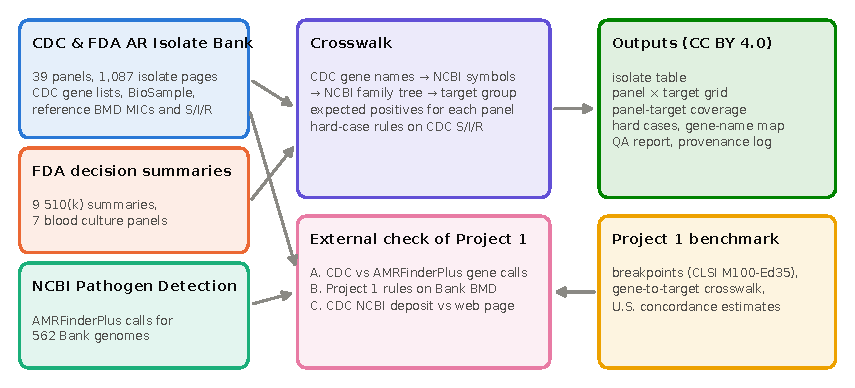
\includegraphics[width=0.92\textwidth]{figures/fig1_design.pdf}
\caption{Study design. Public CDC, FDA and NCBI sources feed two products: the crosswalk of Bank isolates to rapid panel
targets, and an external check of the Project 1 benchmark. BMD, broth microdilution.}
\label{fig:design}
\end{figure*}


Multiplex blood culture identification panels report the organism and a small set of resistance genes within hours of a
positive blood culture \cite{bcid2_2022,verigene2015}. The genes were chosen because each is tied to a treatment
decision: \g{mecA} and its divergent homologue \g{mecC} \cite{garcia2011} for methicillin resistance in \sau{};
\g{vanA} and \g{vanB} for vancomycin resistance in enterococci \cite{courvalin2006}; the carbapenemases KPC, NDM, OXA-48-like, VIM and IMP; CTX-M, the dominant extended-spectrum
$\beta$-lactamase (ESBL) family \cite{bevan2017,bush2020}; and, on newer panels, \g{mcr}, SME and the OXA-23, -24/40 and
-58 carbapenemases of \textit{Acinetobacter}. Molecular rapid diagnostics on positive blood cultures have been
associated with lower mortality and shorter time to effective therapy, particularly with antimicrobial stewardship
\cite{timbrook2017,banerjee2021}.

Before any of these results reaches a patient's chart, the laboratory must show the test works in its hands. Under the
Clinical Laboratory Improvement Amendments, a laboratory that introduces an unmodified FDA-cleared test must, before
reporting patient results, demonstrate performance comparable to the manufacturer's for accuracy, precision and
reportable range \cite{clia}; CLSI has published guidance on verifying commercial microbial identification and susceptibility
systems with characterized isolates \cite{clsim52}. For a resistance-gene
target, accuracy can only be shown with organisms known to carry the target, organisms known not to, and, ideally, the
difficult organisms in which the gene and the growth result disagree.

The CDC \& FDA AR Isolate Bank was created in July 2015 to supply exactly such organisms \cite{lutgring2018}. Its
isolates are characterized by reference broth microdilution and whole-genome sequencing and are offered free to
approved institutions in curated panels \cite{lutgring2018,arbankweb}. CDC reports that in its tenth year the Bank had
grown from 3 to 34 panels and had shipped 500,000 isolates \cite{cdc10yr}. The Bank, however, is organized around
resistance themes (carbapenemase diversity, borderline oxacillin susceptibility, new antibiotics) and around the drugs
whose breakpoints the panels were built to test, not around diagnostic devices. A laboratory bringing up a BioFire BCID2
or a LIAISON PLEX panel has no list of which Bank isolates carry KPC, OXA-48-like or \g{mecC}, and no list of which ones
will look discordant. It must open isolate pages one at a time.

The same isolates also serve a second purpose. The author's U.S. Rapid Panel Resistance Marker Concordance Benchmark
(``Project 1'') measured how often each panel target predicts the susceptibility result reported for U.S. clinical
isolates in NCBI Pathogen Detection \cite{project1}. Its phenotypes come from many submitting laboratories and platforms.
The Bank's results come from one reference laboratory using the reference method, which makes the Bank a natural
external check of that benchmark.

Here we describe the \emph{CDC \& FDA AR Isolate Bank: Rapid Panel Target Crosswalk}, version 1.0.0 \cite{thiswork}. It
(i) captures every Bank isolate's gene list, BioSample accession and reference results exactly as CDC posts them;
(ii) maps CDC's gene names to rapid panel targets through NCBI's gene family tree; (iii) states, for each of
\nv{n-products} FDA-cleared panels, which Bank isolates should be positive for each reported target; (iv) flags hard cases
with explicit rules; and (v) uses the Bank to test the Project 1 benchmark. Section~\ref{sec:methods} describes the
methods, Sec.~\ref{sec:results} the results, Sec.~\ref{sec:discussion} their use and limits, and
Sec.~\ref{sec:conclusions} our conclusions.

% ============================================================================
\section{Materials and methods}\label{sec:methods}

\subsection{Data sources}

All inputs are public (Table~\ref{tab:sources}) and were downloaded on \nv{access-date}. Every file was logged with its
source URL, access date, size and SHA-256 fingerprint (\nv{n-provenance} provenance records).

\begin{table}[t]
\caption{Data sources.}
\label{tab:sources}
\centering\footnotesize
\begin{tabularx}{\linewidth}{@{}>{\raggedright\arraybackslash}p{0.27\linewidth}>{\raggedright\arraybackslash}X@{}}
\toprule
Source & Content used, version and terms \\
\midrule
CDC \& FDA AR Isolate Bank web site & All panel pages and 1,087 isolate pages (AR Bank number, species, BioSample, CDC gene list and calling method, reference broth microdilution MICs and S/I/R, page notes); accessed 24 Oct 2026; U.S.\ government work \\
FDA 510(k) decision summaries & 9 summaries for 7 cleared blood culture panels with resistance targets; U.S.\ government works \\
NCBI Pathogen Detection & AMRFinderPlus genotypes for Bank BioSamples (versions 4.2.5, 4.2.7), streamed from the latest analysis of each organism group; no restrictions on use \\
AMRFinderPlus Reference Gene Hierarchy & Database 2026-08-07.1; gene-to-family tree used to assign targets \\
Project 1 benchmark v1.0.0 & Breakpoint table (CLSI M100-Ed35, checked against FDA STIC), gene-to-target crosswalk, concordance table and isolate list \\
\bottomrule
\end{tabularx}

\end{table}

\subsubsection{Isolate Bank pages}
We downloaded the Bank's \textit{All Isolate Panels} page, every panel page it lists, the \nv{n-panels-linked} custom
panel pages linked from panel descriptions, and every isolate page reached from them (\nv{n-isolate-pages} isolates). The
downloader made one request at a time with a pause between requests and stored each page unchanged. From each isolate
page we read the AR Bank number, species, study identifier, BioSample accession, specimen source, MLST type, the free-text
note CDC sometimes places above the MIC table (for example a cefoxitin disk diffusion result), the MIC table (drug, MIC,
CDC's S/I/R and footnotes), the interpretive standard CDC names for that page, the ``Molecular Mechanisms of
Resistance'' table (category and gene) and CDC's note on how the genes were called. Panel membership was taken from the
panel pages themselves.

\subsubsection{Rapid panel targets}
We took the resistance targets of each FDA-cleared blood culture panel from its 510(k) decision summary
(Table~\ref{tab:products}): BioFire BCID2 \cite{fda_bcid2}, ePlex BCID-GP and BCID-GN \cite{fda_eplexgp,fda_eplexgn},
Verigene BC-GP and BC-GN \cite{fda_vergp,fda_vergn}, and LIAISON PLEX Gram-Positive and Gram-Negative
\cite{fda_lpgp,fda_lpgn}. Each reported target was translated into one or more target groups (for example, BCID2's
``mecA/C'' into \g{mecA} and \g{mecC}; ePlex BCID-GN's ``OXA (OXA-23 and OXA-48 groups only)'' into OXA-23-like and
OXA-48-like). The Verigene BC-GN summary lists ``OXA'' without naming groups; we used the OXA-23 and OXA-48 groups used in
its analytical studies, and the author confirmed this reading.

\begin{table}[t]
\caption{Resistance targets of the FDA-cleared blood culture identification panels included.}
\label{tab:products}
\centering\footnotesize
\begin{tabularx}{\linewidth}{@{}l>{\raggedright\arraybackslash}p{0.2\linewidth}>{\raggedright\arraybackslash}X@{}}
\toprule
Panel & FDA 510(k) & Resistance targets reported \\
\midrule
BioFire BCID2 & K193519 ; K243759 & mecA/C, mecA/C and MREJ (MRSA), vanA/B, CTX-M, KPC, NDM, OXA-48-like, VIM, IMP, mcr-1 \\
ePlex BCID-GP & K181663 & mecA, mecC, vanA, vanB \\
ePlex BCID-GN & K182619 ; K213236 & CTX-M, IMP, KPC, NDM, OXA, VIM \\
Verigene BC-GP & K122514 & mecA, vanA, vanB \\
Verigene BC-GN & K132843 & CTX-M, KPC, NDM, VIM, IMP, OXA \\
LIAISON PLEX GP & K243490 & mecA/mecC, vanA, vanB \\
LIAISON PLEX GN & K243013 & CTX-M, IMP, KPC, MCR, NDM, OXA, SME, VIM \\
\bottomrule
\end{tabularx}

\end{table}

\subsubsection{NCBI gene calls and gene hierarchy}
For the external check we streamed the NCBI Pathogen Detection isolate tables
(\texttt{latest\_snps/AMR/*.amr.metadata.tsv}) for every organism group matching a Bank genus and kept rows whose
BioSample is a Bank BioSample \cite{ncbipd}. These rows carry the AMRFinderPlus genotype NCBI computed for each genome
(versions \nv{amrfinder-versions}) \cite{feldgarden2021}. The AMRFinderPlus Reference Gene Hierarchy (database
\nv{refgene}) was used to place genes in families \cite{feldgarden2021}.

\subsubsection{Project 1 artifacts}
From the Project 1 release we used, unchanged, its breakpoint table (CLSI M100, 35th edition \cite{clsi2025}, checked
against the FDA Susceptibility Test Interpretive Criteria \cite{fdastic}), its AMRFinderPlus-symbol-to-target crosswalk,
its concordance table and its list of benchmark BioSamples \cite{project1}.

\subsection{From CDC gene names to panel targets}

CDC writes allele names without the \textit{bla} prefix (``KPC-3'', ``OXA-232'', ``CTX-M-15''). Each of the
\nv{n-gene-names} distinct names was matched to an NCBI symbol by trying, in order, the name itself, the name with
\textit{bla} added, NCBI synonyms and a case-insensitive match. When a name carried a one-letter bracket note
(``OXA-48(c)''), the note was ignored after real gene names such as \textit{tet}(A) had been tried. The NCBI symbol was
then walked up the Reference Gene Hierarchy until it reached a node that defines a target group: \textit{bla}KPC,
\textit{bla}NDM, \textit{bla}VIM, \textit{bla}IMP, \textit{bla}CTX-M, the \textit{bla}OXA-48, -23, -24, -58 and -143
families, \textit{bla}SME, \g{mcr-1}, \g{mcr-2}, \g{mcr-3}, \g{mecA}, \g{mecC}, \g{vanA} and \g{vanB}. Three rulings were
made by hand and recorded in the released gene map: ``blaZ-mecC'' (the \textit{blaZ} carried on the \g{mecC} element),
which CDC lists for the two isolates of its custom ``\sau{} mecC+'' panel, was counted as \g{mecC}; ``vanHAX (lacks
VanRS)'', which CDC describes on the isolate page as a vancomycin-variable enterococcus, was counted as \g{vanA}; and the
generic entry ``MBL'' was left unmapped because no enzyme is named.

\subsection{Expected positives}

An isolate was marked as an expected positive for a panel's reported target when it carried any target group the
target covers and its organism is one for which the panel reports that target: \g{mecA}/\g{mecC} in staphylococci,
\g{vanA}/\g{vanB} in enterococci, and Gram-negative targets in Enterobacterales, \textit{Pseudomonas} and
\textit{Acinetobacter}. BCID2's MRSA result additionally requires \sau{}; the SCC\textit{mec} right-extremity junction
(MREJ) it detects cannot be read from a gene list, so every \g{mecA}- or \g{mecC}-positive \sau{} was assumed to be an
expected MRSA positive. Fungal, gonococcal, \textit{Clostridioides difficile} and enteric-pathogen panels were listed but
not mapped, because these panels do not report resistance genes for those organisms.

\subsection{Hard cases}

Hard cases were defined on CDC's own posted interpretation, treating intermediate (I) and susceptible-dose-dependent as
not resistant, as in Project 1. Imipenem was not used for \textit{Proteus}, \textit{Morganella} and
\textit{Providencia}, whose imipenem MICs are intrinsically elevated \cite{clsi2025}. The rules were: (1) a target gene is
present and none of the matching drugs is resistant (carbapenems for carbapenemases; ceftriaxone, cefotaxime or
ceftazidime for CTX-M; oxacillin, cefoxitin MIC or, where CDC posts one, cefoxitin disk for \g{mecA}/\g{mecC}; vancomycin
for \g{vanA}/\g{vanB}; colistin for \g{mcr}); (2) an Enterobacterales or \textit{Acinetobacter} isolate is resistant to a
carbapenem without any panel carbapenemase; (3) an Enterobacterales isolate is resistant to a third-generation
cephalosporin without CTX-M or a carbapenemase; (4) a staphylococcus is resistant to oxacillin or cefoxitin without
\g{mecA}/\g{mecC}; and (5) an enterococcus is resistant to vancomycin without \g{vanA}/\g{vanB}. Two patterns in which a
negative panel result is the correct answer were kept as separate categories: carbapenem-resistant \pae{} without a
carbapenemase, usually caused by loss of the OprD porin, efflux and chromosomal AmpC \cite{lister2009}, and enterococci
whose vancomycin resistance comes from intrinsic \g{vanC} \cite{cetinkaya2000}. For rule 2 we classified the other
mechanisms CDC lists, using NCBI's drug subclass for each gene: a carbapenemase not reported by any panel; an intrinsic
OXA-51-like enzyme in \textit{Acinetobacter}; a truncated porin with an ESBL or AmpC; an ESBL or AmpC alone; a truncated
porin alone; or nothing listed.

\subsection{Illustrative verification sets}

To show how the crosswalk can be queried, we computed for each panel the smallest set of Bank isolates whose expected
positives cover all of the panel's reported targets, by a deterministic greedy rule: repeatedly take the isolate that
covers the most uncovered targets, preferring isolates that are not hard cases and then the lowest AR Bank number, using
only isolates in panels on the Bank's main list. This is an example of a query, not a recommended verification protocol.

\subsection{External check of the Project 1 benchmark}

The check used Bank isolates in Project 1's organisms (\sau{}, \textit{E.~faecalis}, \textit{E.~faecium} and
Enterobacterales) that have a BioSample.

\subsubsection{Check A, gene calls}
For Project 1's ten targets, we compared the targets in CDC's gene list with the targets in NCBI's AMRFinderPlus
genotype for the same BioSample, mapped through the Project 1 crosswalk. Agreement is reported as counts and Cohen's
$\kappa$ \cite{cohen1960}. Because some of CDC's gene calls used a database that includes NCBI's, the comparison was
repeated in the isolates CDC called with ResFinder or ARG-ANNOT alone \cite{zankari2012,gupta2014}.

\subsubsection{Check B, gene versus reference result}
CDC's MICs were reinterpreted with Project 1's breakpoint table and censoring rules, and every Project 1 analysis (target,
drug and pooled organism group, with intermediate as not resistant) was recomputed with AMRFinderPlus target calls as the
gene result. Isolates that are also in the Project 1 benchmark were excluded, so the Bank estimates come from isolates
Project 1 never saw. Positive predictive value (PPV), negative predictive value, sensitivity and specificity are reported
with Wilson 95\% intervals \cite{wilson1927} next to Project 1's estimates. Check B used MICs only, as in Project 1; CDC's
cefoxitin disk results enter the hard-case rules but not this comparison.

\subsubsection{Check C, consistency of CDC's records}
For Bank isolates also in the Project 1 benchmark, Project 1's category for each drug (from the antibiogram deposited in
NCBI) was compared with the reinterpreted category from CDC's web page.

\subsection{Reproducibility and quality control}

The pipeline is a set of numbered Python scripts (pandas \cite{mckinney2010}; figures with matplotlib and seaborn
\cite{hunter2007,waskom2021}). Every number in this manuscript is read from files the pipeline writes. A quality-control
report lists row counts, unmatched gene names, every interpretation difference and named spot checks. Before release, the
saved pages were re-parsed with an independently written reader, which matched all \nv{n-mic-rows} MIC rows and
\nv{n-gene-rows} gene rows; all saved pages matched their recorded fingerprints; spot checks were compared with the live
CDC pages; and a clean rebuild from the archived inputs reproduced every released table byte for byte.

\begin{figure*}[t]
\centering
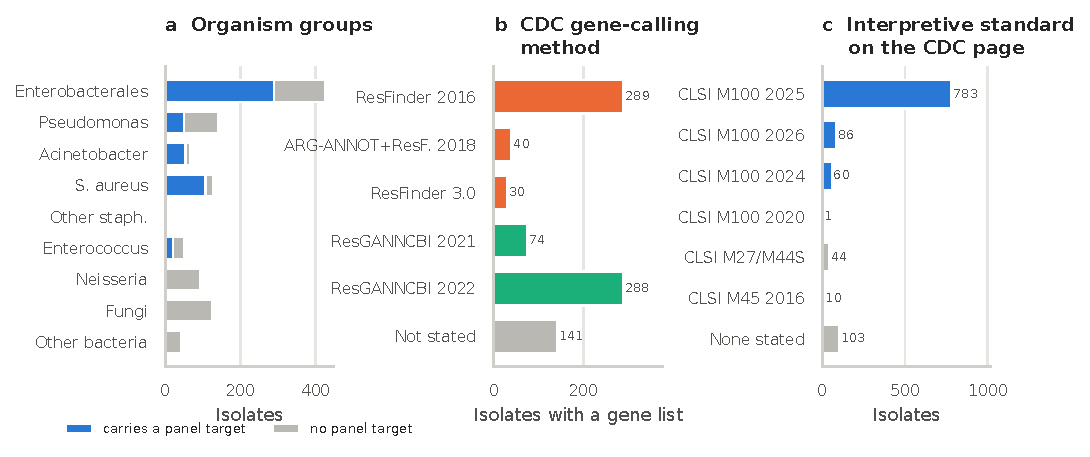
\includegraphics[width=\textwidth]{figures/fig2_collection.pdf}
\caption{The Isolate Bank collection. (a) Isolates by organism group and whether they carry a rapid panel target.
(b) Method CDC states it used to call resistance genes; ResGANNCBI is CDC's combined ResFinder, ARG-ANNOT and NCBI
database. (c) Interpretive standard named on the isolate page.}
\label{fig:collection}
\end{figure*}

\subsection{Ethics}

The study used only public, de-identified data on bacterial and fungal isolates. No human subjects were involved and no
isolates were handled.

% ============================================================================
\section{Results}\label{sec:results}

\subsection{The collection}

The Bank listed \nv{n-panels-listed} panels on its main page, and \nv{n-panels-linked} more custom panels were linked from
their descriptions, for \nv{n-panels} panels and \nv{n-isolates} unique isolates (Table~\ref{tab:collection},
Fig.~\ref{fig:design}). Of these, \nv{n-biosample} list a BioSample accession and \nv{n-mech} list resistance genes.
In all, \nv{n-inscope} isolates belong to organisms that the cleared panels report resistance genes for: \nv{n-grp-ent}
Enterobacterales, \nv{n-grp-psa} \textit{Pseudomonas}, \nv{n-grp-sau} \sau{}, \nv{n-grp-aci} \textit{Acinetobacter},
\nv{n-grp-ent2} enterococci and \nv{n-grp-cons} other staphylococci. The rest are fungi (\nv{n-grp-fungi}),
\textit{Neisseria} (\nv{n-grp-neis}) and other bacteria (\nv{n-grp-oth}), mostly \textit{C.~difficile} and
\textit{Campylobacter}.


\begin{table}[t]
\caption{Isolate Bank collection by organism group. \textit{In scope}: organisms for which a cleared panel reports
resistance genes. \textit{Target}: isolates carrying at least one rapid panel target. \textit{Hard case}: isolates in any
hard-case category, including the two expected-negative categories.}
\label{tab:collection}
\centering\footnotesize
\resizebox{\linewidth}{!}{\begin{tabular}{@{}lrrrcrr@{}}
\toprule
Organism group & Isolates & BioSample & Gene list & In scope & Target & Hard case \\
\midrule
Enterobacterales & 427 & 422 & 408 & yes & 289 & 81 \\
\textit{Pseudomonas} & 140 & 137 & 131 & yes & 50 & 69 \\
\textit{Acinetobacter} & 68 & 68 & 67 & yes & 54 & 6 \\
\textit{S.~aureus} & 129 & 128 & 126 & yes & 107 & 4 \\
Other staphylococci & 9 & 9 & 9 & yes & 8 & 0 \\
\textit{Enterococcus} & 52 & 51 & 50 & yes & 21 & 9 \\
\textit{Neisseria} & 94 & 52 & 19 & no & 0 & 0 \\
Fungi & 126 & 68 & 44 & no & 0 & 0 \\
Other bacteria & 42 & 40 & 8 & no & 0 & 0 \\
\midrule
Total & 1,087 & 975 & 862 & 825 & 529 & 169 \\
\bottomrule
\end{tabular}
}
\end{table}

CDC's pages are not uniform (Fig.~\ref{fig:collection}). Genes were called with ResFinder using its June 2016 database
for \nv{n-meth-resfinder2016} isolates, ARG-ANNOT and ResFinder in 2018 for \nv{n-meth-argannot2018}, ResFinder 3.0 for
\nv{n-meth-resfinder3}, and a combined ResFinder, ARG-ANNOT and NCBI database accessed in 2021 or 2022 for
\nv{n-meth-resgan}; \nv{n-meth-notstated} gene lists name no method. Interpretations cite CLSI M100 2025 for
\nv{n-clsi-2025} isolates, the 2026 edition for \nv{n-clsi-2026}, 2024 for \nv{n-clsi-2024} and 2020 for
\nv{n-clsi-2020}; fungal and fastidious-organism pages cite their own standards, and \nv{n-no-int-std} pages name none.
In addition, \nv{n-fda-footnote} isolate--drug interpretations on \nv{n-fda-footnote-isolates} isolates are footnoted as based on FDA
breakpoints. Of the \nv{n-gene-names} distinct gene names, \nv{n-gene-names-mapped} matched an NCBI symbol and
\nv{n-gene-names-target} mapped to a panel target group; the \nv{n-gene-names-unmapped} unmatched names are mostly point
mutations, efflux genes, porins and fungal targets that no panel reports.


\subsection{Target coverage}

Of the \nv{n-inscope} in-scope isolates, \nv{n-inscope-target} (\nv{pct-inscope-target}) carry at least one panel target,
and \nv{n-multi-target} carry two or more (up to \nv{n-max-targets}). Table~\ref{tab:targets} gives the number of
isolates, panels and species for each target group, and Fig.~\ref{fig:heatmap} shows where they sit. CTX-M is the most
widely represented target (\nv{n-carry-ctx-m} isolates in \nv{n-panels-ctx-m} panels), followed by \g{mecA}
(\nv{n-carry-meca}), KPC (\nv{n-carry-kpc}, \nv{n-panels-kpc} panels), NDM (\nv{n-carry-ndm}), OXA-48-like
(\nv{n-carry-oxa-48like}) and VIM (\nv{n-carry-vim}). The \textit{Acinetobacter} targets reported only by the newer
Gram-negative panels are present (OXA-23-like \nv{n-carry-oxa-23like}, OXA-24/40-like \nv{n-carry-oxa-2440like},
OXA-58-like \nv{n-carry-oxa-58like}), as are SME (\nv{n-carry-sme}) and \g{mcr} genes (\g{mcr-1} \nv{n-carry-mcr-1},
\g{mcr-2} \nv{n-carry-mcr-2}, \g{mcr-3} \nv{n-carry-mcr-3}). \g{mecC} is represented by two isolates (in the borderline-oxacillin panel and its ``mecC+'' custom panel), and OXA-143-like, which LIAISON PLEX Gram-Negative reports, by none.

\begin{table*}[t]
\caption{Rapid panel target groups in the Isolate Bank. \textit{Species} counts distinct genus--species names as CDC
writes them.}
\label{tab:targets}
\centering\footnotesize
\begin{tabularx}{\textwidth}{@{}lrrrl>{\raggedright\arraybackslash}X@{}}
\toprule
Target group & Isolates & Bank panels & Species & Panels reporting it$^{a}$ & CDC allele names (examples) \\
\midrule
mecA & 113 & 6 & 3 & B2, eP, VP, LP & mecA \\
mecC & 2 & 2 & 1 & B2, eP, LP & blaZ-mecC \\
vanA & 11 & 3 & 3 & B2, eP, VP, LP & VanA, vanHAX(lacks VanRs) \\
vanB & 10 & 1 & 2 & B2, eP, VP, LP & VanB \\
KPC & 95 & 16 & 14 & B2, eN, VN, LN & KPC-11, KPC-2, KPC-3, KPC-4, KPC-45, KPC-5, +1 more \\
NDM & 77 & 15 & 12 & B2, eN, VN, LN & NDM, NDM-1, NDM-5, NDM-6, NDM-7 \\
OXA-48-like & 38 & 12 & 7 & B2, eN, VN, LN & OXA-181, OXA-232, OXA-244, OXA-252, OXA-48, OXA-48(c) \\
VIM & 36 & 11 & 4 & B2, eN, VN, LN & VIM, VIM-1, VIM-11, VIM-2, VIM-27, VIM-4, +2 more \\
IMP & 26 & 8 & 7 & B2, eN, VN, LN & IMP-1, IMP-13, IMP-14, IMP-15, IMP-18, IMP-26, +7 more \\
CTX-M & 168 & 17 & 12 & B2, eN, VN, LN & CTX-M-1, CTX-M-124, CTX-M-14, CTX-M-14b, CTX-M-15, CTX-M-2, +6 more \\
OXA-23-like & 28 & 4 & 1 & eN, VN, LN & OXA-23 \\
OXA-24/40-like & 18 & 3 & 1 & LN & OXA-24, OXA-72 \\
OXA-58-like & 3 & 2 & 1 & LN & OXA-58 \\
SME & 9 & 3 & 1 & LN & SME, SME-3, SME-4 \\
mcr-1 & 7 & 1 & 3 & B2, LN & mcr-1 \\
mcr-2 & 1 & 1 & 1 & LN & mcr-2 \\
mcr-3 & 2 & 1 & 2 & LN & mcr-3 \\
\bottomrule
\multicolumn{6}{@{}p{\textwidth}@{}}{\footnotesize $^{a}$B2, BioFire BCID2; eP/eN, ePlex BCID-GP/GN; VP/VN, Verigene BC-GP/GN; LP/LN, LIAISON PLEX Gram-Positive/Gram-Negative. OXA-143-like is reported by LIAISON PLEX GN but no Bank isolate carries it. The MRSA result of BCID2 additionally requires the SCC\textit{mec} right-extremity junction (MREJ), which a gene list cannot show.}\\
\end{tabularx}

\end{table*}

\begin{figure*}[t]
\centering
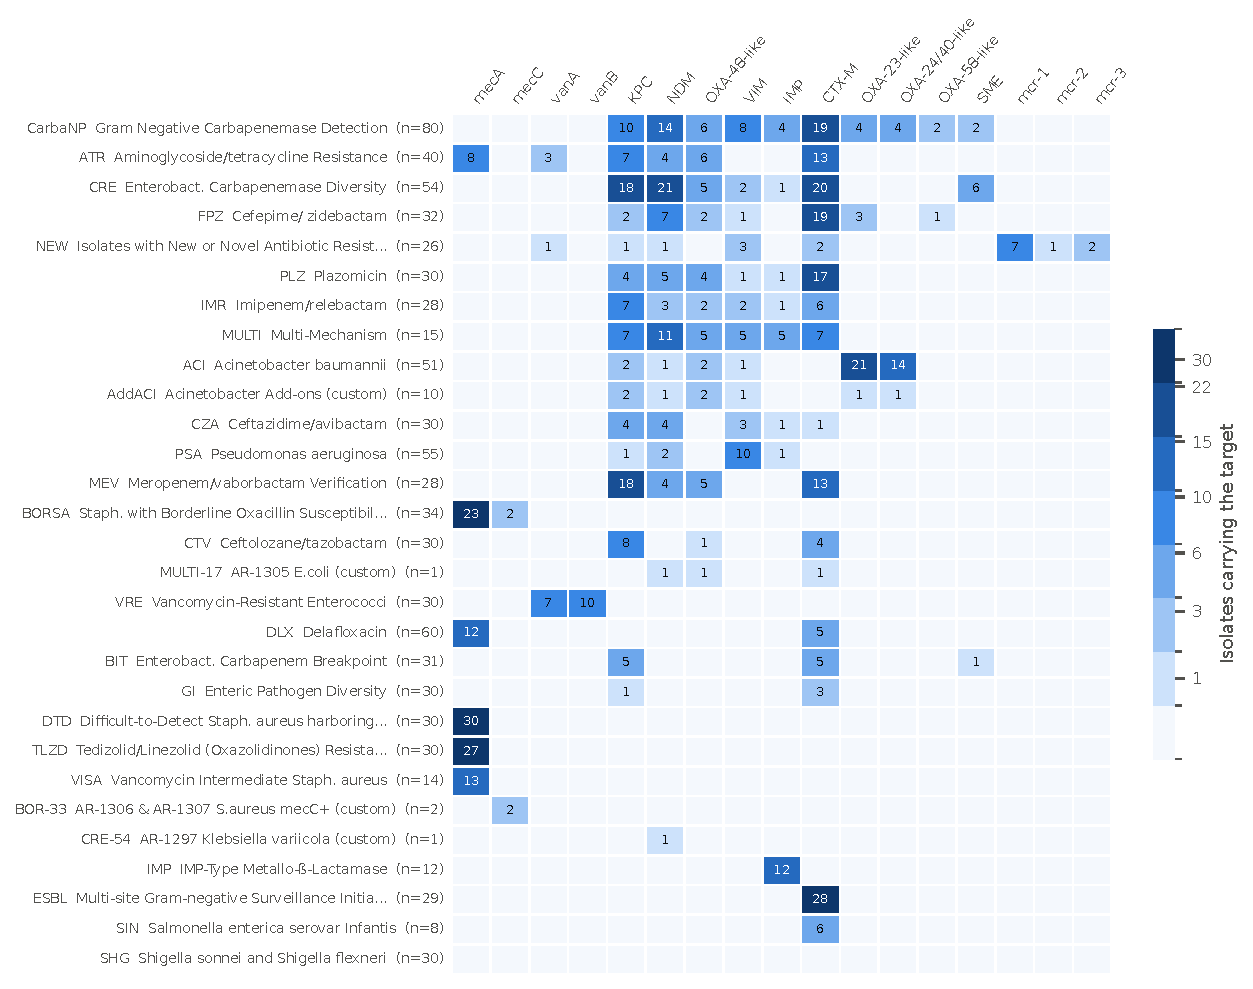
\includegraphics[width=0.94\textwidth]{figures/fig3_heatmap.pdf}
\caption{Isolate Bank panels by rapid panel target. Each cell is the number of isolates in the panel whose CDC gene list
includes the target; blank cells are zero. Panels without organisms that the cleared panels test are omitted. Panel
codes are CDC's; ``custom'' panels are linked from other panels' descriptions. An isolate can belong to several panels.}
\label{fig:heatmap}
\end{figure*}

The panels designed around carbapenemases cover the Gram-negative targets most densely: Gram Negative Carbapenemase
Detection (CarbaNP) holds ten target groups, and Enterobacterales Carbapenemase Diversity (CRE) and the antibiotic
verification panels for cefepime/zidebactam, plazomicin, imipenem/relebactam and meropenem/vaborbactam each hold four to
seven. \g{mecA} sits mainly in the staphylococcal panels (borderline oxacillin susceptibility, difficult-to-detect \g{mecA},
oxazolidinone-resistant staphylococci and vancomycin-intermediate \sau{}), with further isolates in the delafloxacin and
aminoglycoside/tetracycline panels; \g{vanA} and \g{vanB} sit mostly in the VRE panel; and \g{mcr} genes in the panel of
isolates with new or novel resistance.

Fig.~\ref{fig:products} sets the target groups each cleared panel reports against the number of Bank isolates that
carry them, and the released coverage table gives, for each reported target, the expected-positive isolates and their
panels. Every reported target of every panel has at least one expected-positive Bank isolate except
OXA-143-like within LIAISON PLEX's OXA result, which its OXA-23, OXA-24/40, OXA-48 and OXA-58 groups cover. The
greedy query (Table~\ref{tab:verification}) found that \nv{ver-bcid2-n} isolates cover all \nv{ver-bcid2-t} BCID2
resistance targets and \nv{ver-liaisongn-n} cover all \nv{ver-liaisongn-t} LIAISON PLEX Gram-Negative targets; across the
seven panels, between \nv{ver-min} and \nv{ver-max} isolates suffice. Table~\ref{tab:verification} also lists, for each
panel, the expected positives that test not resistant, which a laboratory may want to include deliberately.

\begin{figure*}[t]
\centering
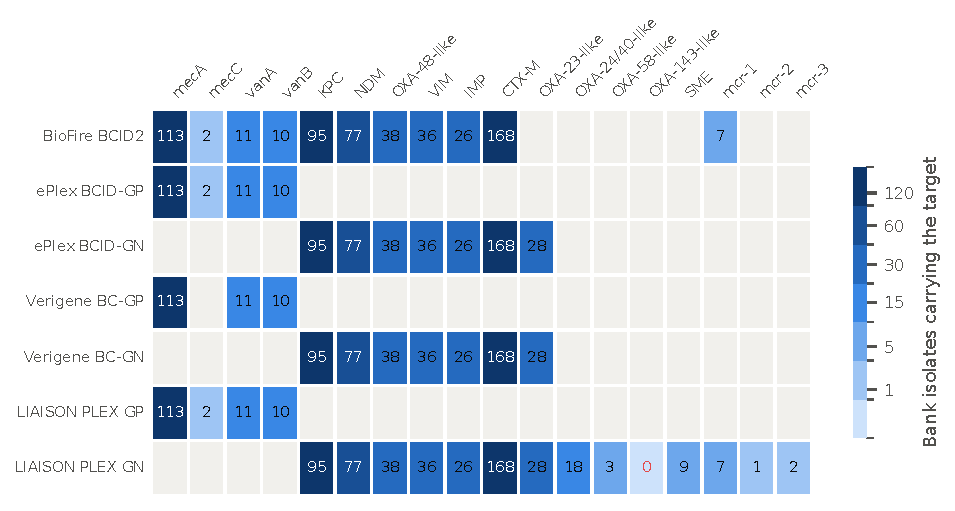
\includegraphics[width=0.86\textwidth]{figures/fig4_products.pdf}
\caption{Rapid panel target groups (columns) reported by each FDA-cleared panel (rows), with the number of Isolate Bank
isolates whose CDC gene list includes the target group. Gray cells: the panel does not report that target group. Several
groups are reported together as one result (for example BCID2's ``mecA/C'' and ``vanA/B'', or ePlex BCID-GN's ``OXA'').
The red 0 marks OXA-143-like, reported by LIAISON PLEX Gram-Negative but carried by no Bank isolate.}
\label{fig:products}
\end{figure*}

\begin{table*}[t]
\caption{Illustrative query: for each panel, the smallest set of Bank isolates (from panels on the Bank's main list) whose
CDC gene lists cover every resistance target the panel reports, chosen by a deterministic greedy rule; and the
expected-positive isolates whose matching drug tests not resistant. This shows how the crosswalk can be used; it is not a
recommended verification protocol, and laboratories should follow the manufacturer's instructions and CLSI M52
\cite{clsim52}.}
\label{tab:verification}
\centering\footnotesize
\begin{tabularx}{\textwidth}{@{}lrr>{\raggedright\arraybackslash}X>{\raggedright\arraybackslash}p{0.2\textwidth}@{}}
\toprule
Panel & Targets & Isolates & Smallest covering set: AR Bank number (targets exercised) & Target present, drug not resistant (AR Bank) \\
\midrule
BioFire BCID2 & 10 & 5 & 1153 (CTX-M, KPC, NDM, OXA-48-like); 0215 (mecA/C, mecA/C and MREJ (MRSA)); 1159 (VIM, IMP); 0346 (mcr-1); 0571 (vanA/B) & 0032, 0050, 0147, 0156, 0451, 0464, 0500, 0541, +5 \\
ePlex BCID-GP & 4 & 4 & 0215 (mecA); 0571 (vanA); 0782 (vanB); 1306 (mecC) & 0464, 0500, 0804, 0998, 1003 \\
ePlex BCID-GN & 6 & 2 & 1153 (CTX-M, KPC, NDM, OXA); 1159 (IMP, VIM) & 0032, 0050, 0147, 0156, 0451, 0541, 0611, 0834 \\
Verigene BC-GP & 3 & 3 & 0215 (mecA); 0571 (vanA); 0782 (vanB) & 0464, 0500, 0804, 0998, 1003 \\
Verigene BC-GN & 6 & 2 & 1153 (CTX-M, KPC, NDM, OXA); 1159 (VIM, IMP) & 0032, 0050, 0147, 0156, 0451, 0541, 0611, 0834 \\
LIAISON PLEX GP & 3 & 3 & 0215 (mecA/mecC); 0571 (vanA); 0782 (vanB) & 0464, 0500, 0804, 0998, 1003 \\
LIAISON PLEX GN & 8 & 4 & 1153 (CTX-M, KPC, NDM, OXA); 1159 (IMP, VIM); 0091 (SME); 0346 (MCR) & 0027, 0032, 0050, 0147, 0156, 0451, 0541, 0611, +1 \\
\bottomrule
\end{tabularx}

\end{table*}

\subsection{Hard cases}

In total, \nv{n-hard} isolates fall into at least one hard-case category (Table~\ref{tab:hardcases}, Fig.~\ref{fig:hardcases});
\nv{n-expected-neg} of them are in the two categories where a negative panel result is expected and
\nv{n-hard-informative} in the others.

\begin{table*}[t]
\caption{Hard cases, by category, on CDC's posted interpretation (intermediate counted as not resistant). An isolate can
fall in more than one category.}
\label{tab:hardcases}
\centering\footnotesize
\begin{tabularx}{\textwidth}{@{}>{\raggedright\arraybackslash}p{0.34\textwidth}r>{\raggedright\arraybackslash}X>{\raggedright\arraybackslash}p{0.17\textwidth}@{}}
\toprule
Category & Isolates & Breakdown & What a laboratory sees \\
\midrule
Target gene present, matching drug(s) not resistant & 14 & KPC 6, mecA 3, VIM 2, SME 1, vanA 1, vanB 1 & Panel positive, AST not resistant \\
Carbapenem resistant, no panel carbapenemase (Enterobacterales, \textit{Acinetobacter}) & 38 & Porin truncation with ESBL or AmpC 16; ESBL or AmpC only 8; No mechanism listed by CDC 5; Carbapenemase not on any panel 4; Intrinsic OXA-51-like (Acinetobacter) 3; Porin truncation only 2 & Panel negative, AST resistant \\
Third-generation cephalosporin resistant, no CTX-M or carbapenemase & 58 & Other ESBL (SHV, TEM), plasmid or chromosomal AmpC & CTX-M negative, AST resistant \\
Oxacillin or cefoxitin resistant, no \textit{mecA}/\textit{mecC} & 1 & No mechanism listed & Panel negative, AST resistant \\
Carbapenem-resistant \textit{P.~aeruginosa}, no carbapenemase & 68 & Chromosomal (OprD, efflux, AmpC) & Expected negative \\
Vancomycin resistant by intrinsic \textit{vanC} & 7 & \textit{E.~gallinarum}, \textit{E.~casseliflavus} & Expected negative \\
\bottomrule
\end{tabularx}

\end{table*}

\begin{figure*}[t]
\centering
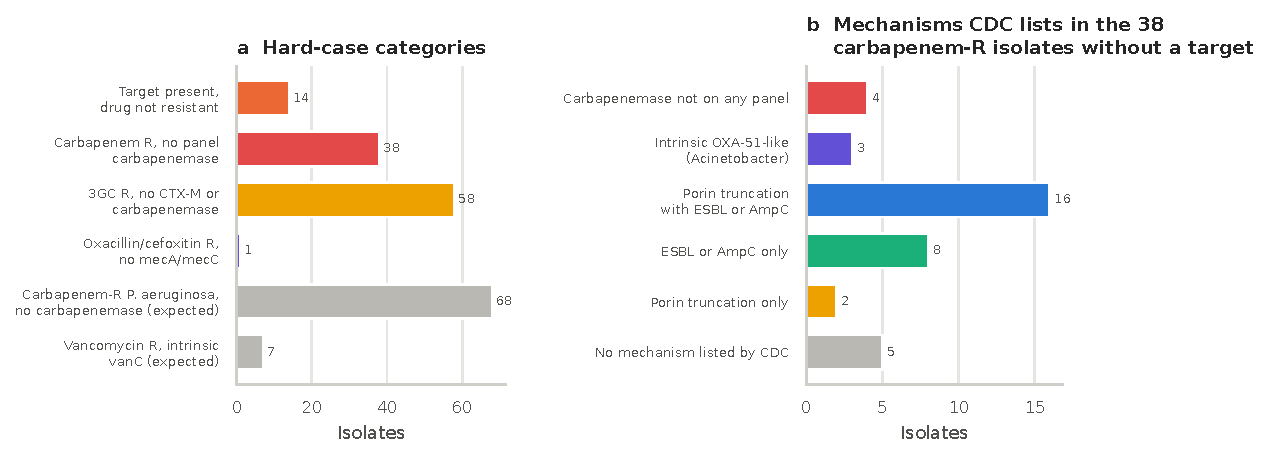
\includegraphics[width=\textwidth]{figures/fig6_hardcases.pdf}
\caption{Hard cases. (a) Isolates in each category; gray bars are the two categories in which a negative panel result is
expected. (b) The mechanisms CDC lists for the \nv{n-hard-carb} carbapenem-resistant Enterobacterales and
\textit{Acinetobacter} without a panel carbapenemase, classified by NCBI drug subclass.}
\label{fig:hardcases}
\end{figure*}

\subsubsection{Target present, drug not resistant}
Table~\ref{tab:tgtnotr} lists the \nv{n-hard-tgt} isolates that carry a panel target while
testing not resistant to every matching drug. Six are KPC producers (KPC-2, -3 or -4) in \textit{E.~cloacae}, \textit{K.~oxytoca},
\textit{E.~coli} and \textit{P.~mirabilis}, with meropenem MICs of 0.25 to 2~mg/L and imipenem and ertapenem MICs
mostly intermediate. Two carry VIM: VIM-1 in \textit{E.~cloacae} (meropenem 1~mg/L) and VIM-11 in \pae{} (all
carbapenems at 4~mg/L, intermediate). One \textit{Serratia marcescens} carries SME with every carbapenem at the lowest
dilution tested. Three \sau{} carry \g{mecA} with oxacillin MICs of 0.25 to 0.5~mg/L and cefoxitin MICs of 4~mg/L
(susceptible); two of them were also susceptible by cefoxitin disk. These resemble oxacillin-susceptible MRSA
\cite{osmrsa2002}. CDC posts a cefoxitin disk result for \nv{n-fox-disk} \g{mecA}-positive \sau{}, of which
\nv{n-dtd-disk-r} are disk resistant; four of these (0977, 0981, 0991, 0992) are susceptible by oxacillin and cefoxitin
MIC, so the disk detects their resistance and they are not counted as hard cases. Among enterococci, the vancomycin-variable \textit{E.~faecium}
0500 carries the \g{vanA} operon without its regulators and tests vancomycin susceptible (1~mg/L)
\cite{szakacs2014,vanA2025}, and \textit{E.~faecalis} 0804 carries \g{vanB} with an intermediate vancomycin MIC of
16~mg/L.

\begin{table*}[t]
\caption{The \nv{n-hard-tgt} isolates that carry a rapid panel target while testing not resistant to every matching drug.
Results are CDC's posted MICs (mg/L), disk diameters (mm) and interpretations.}
\label{tab:tgtnotr}
\centering\footnotesize
\begin{tabularx}{\textwidth}{@{}llll>{\raggedright\arraybackslash}X@{}}
\toprule
AR Bank & Organism & Target & CDC gene & CDC reference results (MIC in mg/L or disk in mm, CDC S/I/R) \\
\midrule
0032 & \textit{Enterobacter cloacae} & KPC & KPC-3 & Meropenem=0.25 S; Imipenem=2 I; Ertapenem=1 I; Doripenem=0.5 S \\
0050 & \textit{Enterobacter cloacae} & KPC & KPC-4 & Meropenem=2 I; Imipenem=2 I; Ertapenem=1 I; Doripenem=0.5 S \\
0147 & \textit{Klebsiella oxytoca} & KPC & KPC-3 & Meropenem=0.5 S; Imipenem=2 I; Ertapenem=1 I; Doripenem=2 I \\
0156 & \textit{Proteus mirabilis} & KPC & KPC-2 & Meropenem=0.25 S; Ertapenem=0.25 S; Doripenem=0.5 S \\
0451 & \textit{Escherichia coli} & KPC & KPC-3 & Meropenem=0.5 S; Imipenem=2 I; Ertapenem=1 I; Doripenem=1 S \\
0541 & \textit{Escherichia coli} & KPC & KPC-3 & Meropenem=1 S; Imipenem=2 I; Ertapenem=1 I; Doripenem=1 S \\
0027 & \textit{Serratia marcescens} & SME & SME & Meropenem=$\le$0.12 S; Imipenem=$\le$0.5 S; Ertapenem=$\le$0.12 S; Doripenem=$\le$0.12 S \\
0611 & \textit{Pseudomonas aeruginosa} & VIM & VIM-11 & Meropenem=4 I; Imipenem=4 I; Doripenem=4 I \\
0834 & \textit{Enterobacter cloacae} & VIM & VIM-1 & Meropenem=1 S; Imipenem=2 I; Ertapenem=0.5 S; Doripenem=2 I \\
0464 & \textit{Staphylococcus aureus} & mecA & mecA & Oxacillin=0.5 S; Cefoxitin=4 S \\
0998 & \textit{Staphylococcus aureus} & mecA & mecA & Oxacillin=$\le$0.25 S; Cefoxitin=4 S; Cefoxitin disk=27 mm S \\
1003 & \textit{Staphylococcus aureus} & mecA & mecA & Oxacillin=0.5 S; Cefoxitin=4 S; Cefoxitin disk=26 mm S \\
0500 & \textit{Enterococcus faecium} & vanA & vanHAX(lacks VanRs) & Vancomycin=1 S \\
0804 & \textit{Enterococcus faecalis} & vanB & VanB & Vancomycin=16 I \\
\bottomrule
\end{tabularx}

\end{table*}

\subsubsection{Meropenem MICs of carbapenemase producers}
Among Enterobacterales with a meropenem result (Fig.~\ref{fig:meropenem}), \nv{mero-ndm-notr} of \nv{mero-ndm-n} NDM
producers and \nv{mero-sme-notr} of \nv{mero-sme-n} SME producers tested not resistant, compared with
\nv{mero-kpc-notr} of \nv{mero-kpc-n} KPC, \nv{mero-oxa48like-notr} of \nv{mero-oxa48like-n} OXA-48-like,
\nv{mero-vim-notr} of \nv{mero-vim-n} VIM and \nv{mero-imp-notr} of \nv{mero-imp-n} IMP producers. No OXA-48-like
producer was meropenem susceptible; all \nv{mero-oxa48like-notr} not-resistant OXA-48-like isolates sat at the
intermediate MIC of 2~mg/L, consistent with the weak carbapenemase activity of this family \cite{poirel2012}. Most of these isolates were resistant to another carbapenem; only the isolates in
Table~\ref{tab:tgtnotr} were not resistant to any.

\begin{figure*}[t]
\centering
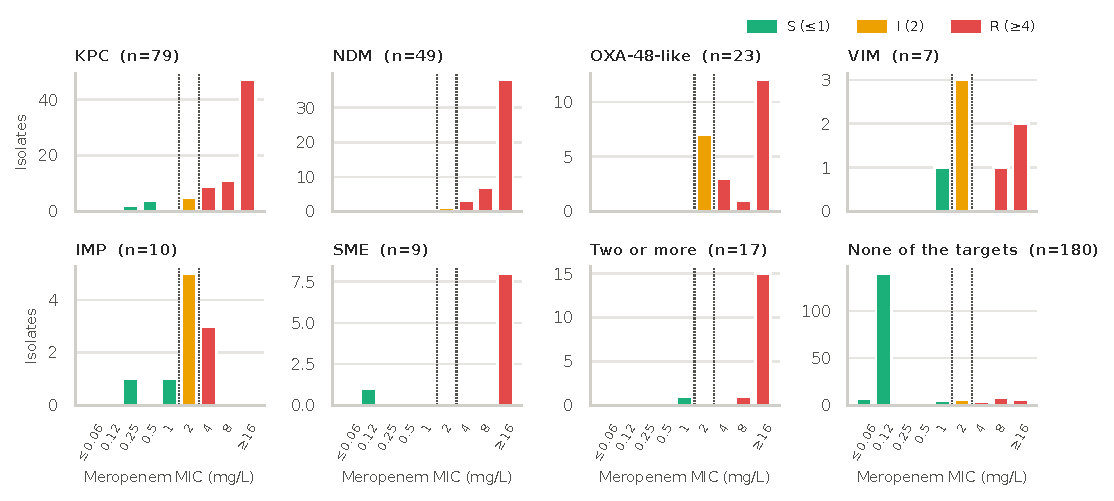
\includegraphics[width=\textwidth]{figures/fig5_meropenem.pdf}
\caption{CDC reference meropenem MICs for Enterobacterales, by the carbapenemase target the isolate carries. Colors give
the CLSI category (susceptible $\le$1, intermediate 2, resistant $\ge$4~mg/L); dotted lines mark the breakpoints. MICs
recorded as $\le$ or $>$ a value are shown at that value.}
\label{fig:meropenem}
\end{figure*}

\subsubsection{Resistant without a target}
Of the \nv{n-hard-carb} carbapenem-resistant Enterobacterales and \textit{Acinetobacter} without a panel carbapenemase,
the largest group (\nv{cm-porinplus}) carry a truncated porin together with an ESBL or AmpC, \nv{cm-esblonly} an ESBL or
AmpC alone and \nv{cm-porinonly} a truncated porin alone (Fig.~\ref{fig:hardcases}b). Another \nv{cm-noncarba} carry a carbapenemase that no cleared panel reports (NMC-A, of the
IMI family, in two \textit{Enterobacter}; OXA-237, of the OXA-134 family, in two \textit{A.~baumannii}), \nv{cm-oxa51}
\textit{A.~baumannii} carry only their intrinsic OXA-51-like enzyme, and for \nv{cm-none} CDC lists no
$\beta$-lactam mechanism. A further \nv{n-hard-esc} Enterobacterales are resistant to a third-generation cephalosporin without CTX-M
or a carbapenemase, typically with SHV or TEM ESBLs or plasmid or chromosomal AmpC enzymes \cite{jacoby2009,bush2020}.
One \sau{} is resistant to oxacillin and cefoxitin without \g{mecA} or \g{mecC}. Of the \nv{n-psa} \pae{} isolates,
\nv{n-psa-target} carry a panel carbapenemase and \nv{n-hard-psa} are carbapenem resistant without one; for these a
negative panel result is the correct answer \cite{lister2009}. Seven \textit{E.~gallinarum} and
\textit{E.~casseliflavus} are vancomycin resistant through intrinsic \g{vanC} \cite{cetinkaya2000}.

\subsection{External check of the Project 1 benchmark}

Of \nv{n-p1org} Bank isolates in Project 1's organisms with a BioSample, \nv{n-ncbi} had AMRFinderPlus results in NCBI
Pathogen Detection and \nv{n-no-ncbi} did not. Of these, \nv{n-overlap} were also in the Project 1 benchmark; all \nv{n-overlap-cdc}
had been deposited in NCBI by CDC itself. They were excluded from check B, leaving \nv{n-indep} independent isolates.

\subsubsection{Check A}
CDC's gene lists and AMRFinderPlus agreed on every isolate for \g{mecA}, \g{mecC}, \g{vanA}, \g{vanB}, KPC, NDM, VIM and
IMP (Table~\ref{tab:checkA}, Fig.~\ref{fig:checkA}). OXA-48-like differed for \nv{ga-oxa-48like-cdconly} isolates, all
\textit{K.~pneumoniae} with OXA-232 listed by CDC and absent from NCBI's analysis ($\kappa$ = \nv{ga-oxa-48like-kappa}), and
CTX-M for \nv{ga-ctx-m-cdconly} in each direction ($\kappa$ = \nv{ga-ctx-m-kappa}). OXA-232 is carried on a small
(6.1~kb) ColE-type plasmid \cite{potron2013}, which may be missing from a public assembly while present in the sequencing
reads; for three of the four isolates CDC states that its calls combined an assembly-based search with SRST2, which
searches the reads directly. NCBI's analysis also confirmed \g{mecC}
in both isolates CDC lists only as ``blaZ-mecC''. Agreement did not depend on CDC's method: \nv{ga-ind-disagree} of
\nv{ga-ind-pos} positive calls differed among isolates CDC called without NCBI's database, and \nv{ga-inc-disagree} of
\nv{ga-inc-pos} among those called with it.

\begin{table}[t]
\caption{Check A: rapid panel targets in CDC's gene lists and in NCBI AMRFinderPlus for the same BioSample. Right-hand
columns restrict to isolates CDC called with ResFinder or ARG-ANNOT alone.}
\label{tab:checkA}
\centering\footnotesize
\resizebox{\linewidth}{!}{\begin{tabular}{@{}lrrrrrrrr@{}}
\toprule
 & \multicolumn{5}{c}{All isolates with both calls} & \multicolumn{3}{c}{CDC method without NCBI database} \\
\cmidrule(lr){2-6}\cmidrule(l){7-9}
Target & $n$ & Both & CDC only & NCBI only & $\kappa$ & $n$ & Both & Disagree \\
\midrule
mecA & 124 & 103 & 0 & 0 & 1.00 & 61 & 51 & 0 \\
mecC & 124 & 2 & 0 & 0 & 1.00 & 61 & 0 & 0 \\
vanA & 39 & 10 & 0 & 0 & 1.00 & 18 & 2 & 0 \\
vanB & 39 & 10 & 0 & 0 & 1.00 & 18 & 0 & 0 \\
KPC & 377 & 74 & 0 & 0 & 1.00 & 161 & 29 & 0 \\
NDM & 377 & 62 & 0 & 0 & 1.00 & 161 & 36 & 0 \\
OXA-48-like & 377 & 30 & 4 & 0 & 0.93 & 161 & 14 & 1 \\
VIM & 377 & 8 & 0 & 0 & 1.00 & 161 & 2 & 0 \\
IMP & 377 & 10 & 0 & 0 & 1.00 & 161 & 1 & 0 \\
CTX-M & 377 & 160 & 2 & 2 & 0.98 & 161 & 63 & 2 \\
\bottomrule
\end{tabular}
}
\end{table}

\begin{figure*}[t]
\centering
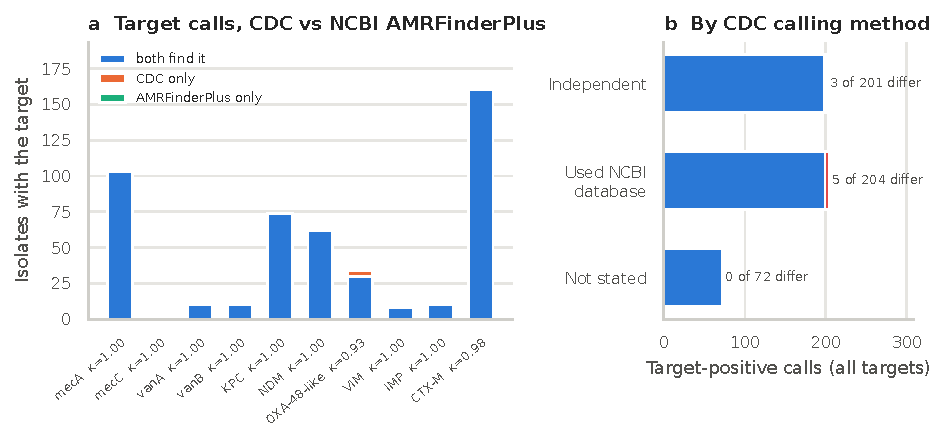
\includegraphics[width=0.94\textwidth]{figures/fig7_checkA.pdf}
\caption{Check A. (a) Isolates in which CDC, NCBI AMRFinderPlus, or both found each target, with Cohen's $\kappa$.
(b) Disagreeing target-positive calls by CDC's gene-calling method; ``independent'' means CDC used ResFinder or ARG-ANNOT
without NCBI's database.}
\label{fig:checkA}
\end{figure*}

\subsubsection{Check B}
Project 1's breakpoint rules reproduced CDC's posted category for \nv{reint-agree} of \nv{n-reint-comp} comparable
isolate--drug results; the \nv{n-reint-dis} differences (Table~\ref{tab:reint}) concern Morganellaceae meropenem and
ceftazidime MICs at the breakpoint, an \textit{Enterobacter} ceftazidime MIC of 8~mg/L, and one \g{mecA}-positive \sau{}
with an oxacillin MIC of 2~mg/L that CDC reports as resistant, as CLSI directs for \g{mecA}-positive isolates
\cite{clsi2025}.

Table~\ref{tab:checkB} and Fig.~\ref{fig:checkB} set the Bank estimates beside Project 1's. When a target gene was
present, the share of isolates testing resistant was similar to Project 1 for the high-PPV targets: KPC predicted
resistance to any carbapenem in \nv{b-kpc-any-ppv-frac} (\nv{b-kpc-any-ppv}; Project 1 \nv{p1-kpc-any-ppv}), OXA-48-like in \nv{b-oxa-any-ppv-frac}
(\nv{b-oxa-any-ppv}), the five panel carbapenemases together in \nv{b-carb-any-ppv-frac} (\nv{b-carb-any-ppv}; Project 1
\nv{p1-carb-any-ppv}), and CTX-M predicted ceftriaxone resistance in \nv{b-ctx-cro-ppv-frac} (\nv{b-ctx-cro-ppv}; Project
1 \nv{p1-ctx-cro-ppv}). The drug-level pattern also held: carbapenemase producers were less often resistant to meropenem
(PPV \nv{b-carb-mero-ppv}) than to any carbapenem, and OXA-48-like producers least of all (\nv{b-oxa-mero-ppv-frac}
meropenem resistant). For CTX-M and ceftazidime the Bank PPV was higher than Project 1's (\nv{b-ctx-caz-ppv} versus
\nv{p1-ctx-caz-ppv}).

The measures that depend on what else is in the collection differed, as expected. Among \sau{}, \g{mecA}-positive
isolates were often oxacillin susceptible by MIC (\nv{b-meca-ox-genepos-notr} of them), so specificity for oxacillin was
\nv{b-meca-ox-spec} against Project 1's \nv{p1-meca-ox-specificity}; with cefoxitin added, PPV was \nv{b-meca-oxfox-ppv}
and specificity \nv{b-meca-oxfox-spec}. These are the Bank's deliberately difficult staphylococci: its borderline
oxacillin (BORSA) and difficult-to-detect \g{mecA} (DTD) panels. Sensitivity of each single carbapenemase was low because
Bank isolates carry many different carbapenemases, but sensitivity of the five together for any-carbapenem resistance was
\nv{b-carb-any-sens} (Project 1 \nv{p1-carb-any-sensitivity}) and for meropenem \nv{b-carb-mero-sens} (Project 1
\nv{p1-carb-mero-sensitivity}). CTX-M sensitivity for ceftriaxone resistance matched Project 1 (\nv{b-ctx-cro-sens} versus
\nv{p1-ctx-cro-sensitivity}), confirming that a negative CTX-M result is a weak predictor of ceftriaxone susceptibility.

\begin{table*}[t]
\caption{Check B: Project 1 rules applied to independent Bank isolates (Bank) beside Project 1's U.S. estimates (P1).
$n$ is Bank isolates with an interpretable result; PPV and sensitivity also give Bank counts. Enterobacterales exclude
\textit{Salmonella}; enterococci are \textit{E.~faecalis} and \textit{E.~faecium}. -- , not estimable.}
\label{tab:checkB}
\centering\footnotesize
\begin{tabular}{@{}llrrrrrrrrr@{}}
\toprule
 & & & \multicolumn{3}{c}{PPV} & \multicolumn{3}{c}{Sensitivity} & \multicolumn{2}{c}{Specificity} \\
\cmidrule(lr){4-6}\cmidrule(lr){7-9}\cmidrule(l){10-11}
Target & Drug & $n$ & Bank & Bank & P1 & Bank & Bank & P1 & Bank & P1 \\
\midrule
mecA & oxacillin & 127 & 67/103 & 65.0\% & 97.7\% & 67/68 & 98.5\% & 100.0\% & 39.0\% & 98.5\% \\
mecA & cefoxitin & 127 & 97/103 & 94.2\% & -- & 97/100 & 97.0\% & 0.0\% & 77.8\% & -- \\
mecA & oxacillin or cefoxitin & 127 & 97/103 & 94.2\% & 97.7\% & 97/100 & 97.0\% & 99.5\% & 77.8\% & 98.5\% \\
vanA & vancomycin & 41 & 9/10 & 90.0\% & 89.7\% & 9/18 & 50.0\% & 89.7\% & 95.7\% & 96.7\% \\
vanB & vancomycin & 41 & 9/10 & 90.0\% & -- & 9/18 & 50.0\% & 0.0\% & 95.7\% & 100.0\% \\
KPC & meropenem & 312 & 54/64 & 84.4\% & 90.5\% & 54/148 & 36.5\% & 55.3\% & 93.9\% & 99.5\% \\
KPC & any carbapenem & 312 & 60/64 & 93.8\% & 98.0\% & 60/178 & 33.7\% & 47.0\% & 97.0\% & 99.9\% \\
NDM & meropenem & 312 & 52/53 & 98.1\% & 97.6\% & 52/148 & 35.1\% & 12.2\% & 99.4\% & 100.0\% \\
NDM & any carbapenem & 312 & 53/53 & 100.0\% & 100.0\% & 53/178 & 29.8\% & 9.7\% & 100.0\% & 100.0\% \\
OXA-48-like & meropenem & 312 & 19/26 & 73.1\% & 76.3\% & 19/148 & 12.8\% & 8.8\% & 95.7\% & 99.7\% \\
OXA-48-like & any carbapenem & 312 & 26/26 & 100.0\% & 94.7\% & 26/178 & 14.6\% & 8.5\% & 100.0\% & 100.0\% \\
VIM & meropenem & 312 & 3/6 & 50.0\% & 75.0\% & 3/148 & 2.0\% & 0.9\% & 98.2\% & 100.0\% \\
IMP & meropenem & 312 & 1/3 & 33.3\% & 37.5\% & 1/148 & 0.7\% & 0.9\% & 98.8\% & 99.9\% \\
CTX-M & ceftriaxone & 350 & 146/146 & 100.0\% & 97.7\% & 146/264 & 55.3\% & 56.5\% & 100.0\% & 99.1\% \\
CTX-M & ceftazidime & 312 & 127/145 & 87.6\% & 57.0\% & 127/235 & 54.0\% & 42.7\% & 76.6\% & 86.7\% \\
\midrule
mecA or mecC & oxacillin or cefoxitin & 127 & 99/105 & 94.3\% & 97.7\% & 99/100 & 99.0\% & 99.5\% & 77.8\% & 98.5\% \\
vanA or vanB & vancomycin & 41 & 18/20 & 90.0\% & 89.7\% & 18/18 & 100.0\% & 89.7\% & 91.3\% & 96.7\% \\
Any of 5 carbapenemases & meropenem & 312 & 124/147 & 84.4\% & 87.6\% & 124/148 & 83.8\% & 73.2\% & 86.0\% & 99.0\% \\
Any of 5 carbapenemases & any carbapenem & 312 & 142/147 & 96.6\% & 97.8\% & 142/178 & 79.8\% & 64.3\% & 96.3\% & 99.8\% \\
\bottomrule
\end{tabular}

\end{table*}

\begin{figure*}[t]
\centering
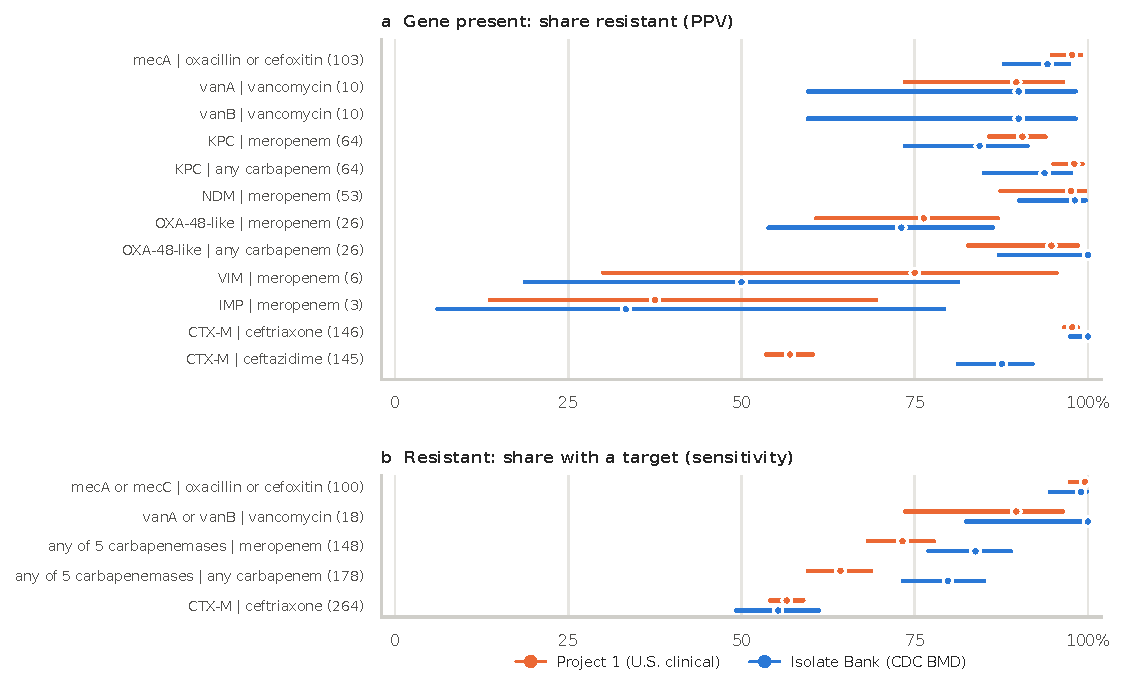
\includegraphics[width=0.8\textwidth]{figures/fig8_checkB.pdf}
\caption{Check B. (a) Share of gene-positive isolates that test resistant (PPV) and (b) share of resistant isolates that
carry a target (sensitivity), Bank (blue) beside Project 1 (orange), with 95\% Wilson intervals. Numbers in brackets are
Bank denominators.}
\label{fig:checkB}
\end{figure*}

\begin{table}[t]
\caption{The \nv{n-reint-dis} isolate--drug results where Project 1's breakpoint rules and CDC's posted category differ.}
\label{tab:reint}
\centering\footnotesize
\resizebox{\linewidth}{!}{\begin{tabular}{@{}lllrcc@{}}
\toprule
AR Bank & Organism group & Drug & MIC & CDC & Project 1 rules \\
\midrule
0057 & Morganella / Providencia & meropenem & 2 & R & I \\
0082 & Morganella / Providencia & meropenem & 4 & I & R \\
0155 & Morganella / Providencia & ceftazidime & 8 & R & I \\
0216 & \textit{Staphylococcus aureus} & oxacillin & 2 & R & S \\
1011 & \textit{Enterobacter cloacae} complex & ceftazidime & 8 & R & I \\
1113 & Morganella / Providencia & meropenem & 2 & S & I \\
\bottomrule
\end{tabular}
}
\end{table}

\subsubsection{Check C}
For the \nv{n-cons-pairs} isolate--drug results on the \nv{n-overlap} overlapping isolates, the category from CDC's NCBI
antibiogram matched the category from CDC's web page in \nv{cons-agree}, with \nv{n-cons-major} major or very major
differences; the \nv{n-cons-dis} differences were susceptible versus intermediate at a carbapenem breakpoint. Because both
records come from CDC, this is a consistency check of CDC's two postings, not a comparison between laboratories.

% ============================================================================
\section{Discussion}\label{sec:discussion}

\subsection{Principal findings}

The Isolate Bank already contains reference organisms for nearly every resistance target reported by the seven FDA-cleared
blood culture panels with resistance targets, and for most of the ways those targets can mislead. What it lacked was an
index by target and by device. The crosswalk supplies it: each isolate's targets, the panels that should call it positive,
its reference results, and whether it is a hard case. Two to five isolates cover every target of any one panel, and the
hard-case list offers a further set of organisms that tests what a panel cannot know.

Used as an external yardstick, the Bank supports the Project 1 benchmark where the benchmark is meant to be read. Gene
calls by two different pipelines agreed almost perfectly. The benchmark's breakpoint rules reproduced CDC's reference
interpretations. And the quantities that describe the gene itself (how often a gene-positive isolate is resistant, and
to which carbapenem) behaved the same way in reference broth microdilution data from one laboratory as in submitted
results from many.

\subsection{Using the crosswalk for verification}

A laboratory verifying a panel can filter the released isolate table by the panel's \texttt{expected\_positive} column to
see every candidate positive, by \texttt{hard\_case\_types} to find challenge organisms, and by organism to find negative
controls of the right species. The covering sets in Table~\ref{tab:verification} show that coverage is cheap; the
hard-case list is where the crosswalk adds most. A KPC-producing \textit{E.~coli} with a meropenem MIC of 0.5~mg/L, a
\g{mecA}-positive \sau{} susceptible by oxacillin and cefoxitin MIC, or a vancomycin-susceptible \textit{E.~faecium}
carrying \g{vanA} will each produce a positive panel result and a susceptible AST result. Including them in a
verification shows the laboratory and its stewardship program what such a result looks like before it happens on a
patient isolate, and tests whether the laboratory's reporting rules (for example, reporting \g{mecA}-positive \sau{} as
oxacillin resistant \cite{clsi2025}) are applied. Conversely, the carbapenem-resistant isolates without a panel
carbapenemase, and especially the NMC-A, OXA-237 and porin-loss isolates, show the limits of a negative carbapenemase
result \cite{tamma2017,pitout2015}.

\subsection{What the external check shows}

The check separates measures that describe a gene from measures that describe a population. PPV for KPC, NDM and
OXA-48-like against any carbapenem, and for CTX-M against ceftriaxone, had overlapping 95\% ranges in the Bank and
in Project 1, and
the low meropenem PPV of OXA-48-like producers reappeared in reference broth microdilution data \cite{poirel2012}.
Specificity for \g{mecA} and single-gene sensitivities, in contrast, were lower in the Bank because the Bank was built to
contain the exceptions: borderline and difficult-to-detect staphylococci, and carbapenem-resistant Enterobacterales with
every mechanism CDC could collect. These differences are therefore not evidence against Project 1's estimates for U.S.
clinical isolates; they show what those estimates look like in a challenge set. The higher CTX-M PPV for ceftazidime in the Bank
than in Project 1 may reflect the Bank's many multi-mechanism isolates; we did not test this.

\subsection{Limitations}

The crosswalk records which targets an isolate carries, not whether a particular assay detects that allele; detection is
defined by each manufacturer's instructions for use. The MRSA result of BCID2 depends on the MREJ junction, which a gene
list cannot show, so its expected positives are an assumption. The Verigene BC-GN OXA groups are not named by FDA and were
taken from its analytical studies. CDC's gene lists came from several methods between 2016 and 2022, and older calls can
miss genes added to databases later; the gene-call comparison is only partly independent of NCBI, although agreement was as
high in the independent subset. Hard cases rest on CDC's posted interpretations, which cite four CLSI M100 editions, while
the external check uses a single breakpoint table. The Bank is not a patient population, so its prevalence-dependent
measures should not be compared directly with clinical estimates. Some targets are represented by few isolates
(\g{mecC} by two, OXA-58-like by three) and OXA-143-like by none. Thirty-one Bank isolates in Project 1's organisms had no
NCBI AMRFinderPlus result and \nv{n-no-biosample} isolates list no BioSample. The release reflects the Bank's pages on
\nv{access-date}; CDC adds isolates and revises MICs, so the crosswalk will need yearly refresh. No isolates were tested.

\section{Conclusions}\label{sec:conclusions}

An open, versioned crosswalk turns the CDC \& FDA AR Isolate Bank into a target-by-target, device-by-device catalog for
verifying rapid blood culture panels: \nv{n-inscope-target} isolates carry a panel target, every target but one is
represented, a handful of isolates covers each panel, and \nv{n-hard-informative} isolates are flagged as hard cases
outside the expected-negative groups. Used as an external reference-method check, the Bank confirmed the gene calls,
interpretation rules and gene-level estimates of a U.S. genotype--phenotype benchmark. Both resources are released for
reuse and will be refreshed as the Bank grows.

% ============================================================================
\section*{Data and code availability}
\addcontentsline{toc}{section}{Data and code availability}
All data, code and documentation are available at
\url{https://github.com/FatimaAbdulwahab/ar-isolate-bank-panel-crosswalk} \cite{thiswork}: the isolate-level crosswalk,
the panel-by-target grid, panel target coverage, the hard-case list, the CDC gene-name map, the rapid panel target table
with FDA sources, the external-check outputs, a codebook, a limitations file, the quality-control report and a provenance
log with source URLs, access dates, sizes and SHA-256 fingerprints. The CDC pages, NCBI rows and FDA documents used are
archived in the repository, and \texttt{run\_all.sh} rebuilds every result from them. Data and documents are released under
CC BY 4.0 and code under the MIT license. The Project 1 benchmark is at
\url{https://github.com/FatimaAbdulwahab/us-rapid-panel-amr-concordance} \cite{project1}.

\section*{Author contributions}
F.A.: conceptualization, methodology, data curation, formal analysis, validation, visualization, writing (original draft,
review and editing).

\section*{Competing interests}
The author declares no competing interests and no relationship with CDC, FDA or any manufacturer of rapid diagnostic
panels. This work is not affiliated with or endorsed by CDC or FDA.

\section*{Funding}
This work received no specific funding.

\section*{Use of AI tools}
Claude (Anthropic) assisted with code, data processing, figure generation and drafting of this manuscript. The author
made the analytic decisions and rulings, verified the outputs against the CDC, FDA and NCBI records, and takes
responsibility for the content.

\section*{Acknowledgments}
The author thanks CDC's Division of Healthcare Quality Promotion and FDA for building and maintaining the Antimicrobial
Resistance Isolate Bank and publishing its characterization data, and the NCBI Pathogen Detection team for AMRFinderPlus
and the Reference Gene Catalog.

\small
% Auto-generated by make_refs.py from Crossref records (crossref_raw.json). Do not edit.
\begin{thebibliography}{43}
\bibitem{bcid2_2022} Anna Maria Peri et al. Performance of BioFire Blood Culture Identification 2 Panel (BCID2) for the detection of bloodstream pathogens and their associated resistance markers: a systematic review and meta-analysis of diagnostic test accuracy studies. \textit{BMC Infect Dis}, 22(1):794, 2022. \href{https://doi.org/10.1186/s12879-022-07772-x}{doi:10.1186/s12879-022-07772-x}

\bibitem{verigene2015} Naoki Uno et al. Multicenter evaluation of the Verigene Gram-negative blood culture nucleic acid test for rapid detection of bacteria and resistance determinants in positive blood cultures. \textit{Diagnostic Microbiology and Infectious Disease}, 83(4):344-348, 2015. \href{https://doi.org/10.1016/j.diagmicrobio.2015.08.004}{doi:10.1016/j.diagmicrobio.2015.08.004}

\bibitem{garcia2011} Laura García-Álvarez et al. Meticillin-resistant \textit{Staphylococcus aureus} with a novel mecA homologue in human and bovine populations in the UK and Denmark: a descriptive study. \textit{The Lancet Infectious Diseases}, 11(8):595-603, 2011. \href{https://doi.org/10.1016/s1473-3099(11)70126-8}{doi:10.1016/s1473-3099(11)70126-8}

\bibitem{courvalin2006} Patrice Courvalin. Vancomycin Resistance in Gram-Positive Cocci. \textit{Clinical Infectious Diseases}, 42(Suppl.~1):S25-S34, 2006. \href{https://doi.org/10.1086/491711}{doi:10.1086/491711}

\bibitem{bevan2017} Edward R. Bevan, Annie M. Jones, and Peter M. Hawkey. Global epidemiology of CTX-M $\beta$-lactamases: temporal and geographical shifts in genotype. \textit{Journal of Antimicrobial Chemotherapy}, 72(8):2145-2155, 2017. \href{https://doi.org/10.1093/jac/dkx146}{doi:10.1093/jac/dkx146}

\bibitem{bush2020} Karen Bush and Patricia A. Bradford. Epidemiology of $\beta$-Lactamase-Producing Pathogens. \textit{Clin Microbiol Rev}, 33(2):e00047-19, 2020. \href{https://doi.org/10.1128/cmr.00047-19}{doi:10.1128/cmr.00047-19}

\bibitem{timbrook2017} Tristan T. Timbrook et al. The Effect of Molecular Rapid Diagnostic Testing on Clinical Outcomes in Bloodstream Infections: A Systematic Review and Meta-analysis. \textit{Clin Infect Dis.}, 64(1):15-23, 2017. \href{https://doi.org/10.1093/cid/ciw649}{doi:10.1093/cid/ciw649}

\bibitem{banerjee2021} Ritu Banerjee and Romney Humphries. Rapid Antimicrobial Susceptibility Testing Methods for Blood Cultures and Their Clinical Impact. \textit{Front. Med.}, 8:635831, 2021. \href{https://doi.org/10.3389/fmed.2021.635831}{doi:10.3389/fmed.2021.635831}

\bibitem{clia} Code of Federal Regulations. Title 42, \S\,493.1253, Standard: Establishment and verification of performance specifications. \url{https://www.ecfr.gov/current/title-42/section-493.1253}.

\bibitem{clsim52} Clinical and Laboratory Standards Institute. \textit{Verification of Commercial Microbial Identification and Antimicrobial Susceptibility Testing Systems}. CLSI guideline M52, 1st edition. Clinical and Laboratory Standards Institute, Wayne, PA, 2015.

\bibitem{lutgring2018} Joseph D. Lutgring et al. FDA-CDC Antimicrobial Resistance Isolate Bank: a Publicly Available Resource To Support Research, Development, and Regulatory Requirements. \textit{J Clin Microbiol}, 56(2):e01415-17, 2018. \href{https://doi.org/10.1128/jcm.01415-17}{doi:10.1128/jcm.01415-17}

\bibitem{arbankweb} Centers for Disease Control and Prevention and U.S. Food and Drug Administration. CDC \& FDA Antimicrobial Resistance Isolate Bank. \url{https://wwwn.cdc.gov/ARIsolateBank/}. Accessed 24 October 2026.

\bibitem{cdc10yr} Centers for Disease Control and Prevention. \textit{CDC \& FDA Antimicrobial Resistance Isolate Bank: 10 Facts for 10 Years}. CDC, Atlanta, GA, revised January 2026. \url{https://www.cdc.gov/antimicrobial-resistance/media/pdfs/10-Facts-for-10-Years-508.pdf}.

\bibitem{project1} Fatima Abdulwahab. U.S. Rapid Panel Resistance Marker Concordance Benchmark, version 1.0.0. \url{https://github.com/FatimaAbdulwahab/us-rapid-panel-amr-concordance}, 2026.

\bibitem{thiswork} Fatima Abdulwahab. CDC \& FDA Antimicrobial Resistance Isolate Bank: Rapid Panel Target Crosswalk, version 1.0.0. \url{https://github.com/FatimaAbdulwahab/ar-isolate-bank-panel-crosswalk}, 2026. Archived on Zenodo.

\bibitem{fda_bcid2} U.S. Food and Drug Administration. 510(k) decision summaries K193519 and K243759, BIOFIRE Blood Culture Identification 2 (BCID2) Panel. \url{https://www.accessdata.fda.gov/cdrh_docs/reviews/K193519.pdf}.

\bibitem{fda_eplexgp} U.S. Food and Drug Administration. 510(k) decision summary K181663, ePlex Blood Culture Identification Gram-Positive (BCID-GP) Panel. \url{https://www.accessdata.fda.gov/cdrh_docs/reviews/K181663.pdf}.

\bibitem{fda_eplexgn} U.S. Food and Drug Administration. 510(k) decision summaries K182619 and K213236, ePlex Blood Culture Identification Gram-Negative (BCID-GN) Panel. \url{https://www.accessdata.fda.gov/cdrh_docs/reviews/K182619.pdf}.

\bibitem{fda_vergp} U.S. Food and Drug Administration. 510(k) summary K122514, Verigene Gram-Positive Blood Culture Nucleic Acid Test (BC-GP). \url{https://www.accessdata.fda.gov/cdrh_docs/pdf12/K122514.pdf}.

\bibitem{fda_vergn} U.S. Food and Drug Administration. 510(k) decision summary K132843, Verigene Gram-Negative Blood Culture Nucleic Acid Test (BC-GN). \url{https://www.accessdata.fda.gov/cdrh_docs/reviews/K132843.pdf}.

\bibitem{fda_lpgp} U.S. Food and Drug Administration. 510(k) decision summary K243490, LIAISON PLEX Gram-Positive Blood Culture Assay. \url{https://www.accessdata.fda.gov/cdrh_docs/reviews/K243490.pdf}.

\bibitem{fda_lpgn} U.S. Food and Drug Administration. 510(k) decision summary K243013, LIAISON PLEX Gram-Negative Blood Culture Assay. \url{https://www.accessdata.fda.gov/cdrh_docs/reviews/K243013.pdf}.

\bibitem{ncbipd} National Center for Biotechnology Information. Pathogen Detection. \url{https://www.ncbi.nlm.nih.gov/pathogens/}. Data accessed 24 October 2026.

\bibitem{feldgarden2021} Michael Feldgarden et al. AMRFinderPlus and the Reference Gene Catalog facilitate examination of the genomic links among antimicrobial resistance, stress response, and virulence. \textit{Sci Rep}, 11(1):12728, 2021. \href{https://doi.org/10.1038/s41598-021-91456-0}{doi:10.1038/s41598-021-91456-0}

\bibitem{clsi2025} Clinical and Laboratory Standards Institute. \textit{Performance Standards for Antimicrobial Susceptibility Testing}. CLSI supplement M100, 35th edition. Clinical and Laboratory Standards Institute, Wayne, PA, 2025.

\bibitem{fdastic} U.S. Food and Drug Administration. Antibacterial Susceptibility Test Interpretive Criteria. \url{https://www.fda.gov/drugs/development-resources/antibacterial-susceptibility-test-interpretive-criteria}. Accessed 24 October 2026.

\bibitem{lister2009} Philip D. Lister, Daniel J. Wolter, and Nancy D. Hanson. Antibacterial-Resistant \textit{Pseudomonas aeruginosa} : Clinical Impact and Complex Regulation of Chromosomally Encoded Resistance Mechanisms. \textit{Clin Microbiol Rev}, 22(4):582-610, 2009. \href{https://doi.org/10.1128/cmr.00040-09}{doi:10.1128/cmr.00040-09}

\bibitem{cetinkaya2000} Yesim Cetinkaya, Pamela Falk, and C. Glen Mayhall. Vancomycin-Resistant Enterococci. \textit{Clin Microbiol Rev}, 13(4):686-707, 2000. \href{https://doi.org/10.1128/cmr.13.4.686}{doi:10.1128/cmr.13.4.686}

\bibitem{cohen1960} Jacob Cohen. A Coefficient of Agreement for Nominal Scales. \textit{Educational and Psychological Measurement}, 20(1):37-46, 1960. \href{https://doi.org/10.1177/001316446002000104}{doi:10.1177/001316446002000104}

\bibitem{zankari2012} E. Zankari et al. Identification of acquired antimicrobial resistance genes. \textit{Journal of Antimicrobial Chemotherapy}, 67(11):2640-2644, 2012. \href{https://doi.org/10.1093/jac/dks261}{doi:10.1093/jac/dks261}

\bibitem{gupta2014} Sushim Kumar Gupta et al. ARG-ANNOT, a New Bioinformatic Tool To Discover Antibiotic Resistance Genes in Bacterial Genomes. \textit{Antimicrob Agents Chemother}, 58(1):212-220, 2014. \href{https://doi.org/10.1128/aac.01310-13}{doi:10.1128/aac.01310-13}

\bibitem{wilson1927} Edwin B. Wilson. Probable Inference, the Law of Succession, and Statistical Inference. \textit{Journal of the American Statistical Association}, 22(158):209-212, 1927. \href{https://doi.org/10.1080/01621459.1927.10502953}{doi:10.1080/01621459.1927.10502953}

\bibitem{mckinney2010} Wes McKinney. Data Structures for Statistical Computing in Python. \textit{Proceedings of the Python in Science Conference}, 56--61, 2010. \href{https://doi.org/10.25080/majora-92bf1922-00a}{doi:10.25080/majora-92bf1922-00a}

\bibitem{hunter2007} John D. Hunter. Matplotlib: A 2D Graphics Environment. \textit{Comput. Sci. Eng.}, 9(3):90-95, 2007. \href{https://doi.org/10.1109/mcse.2007.55}{doi:10.1109/mcse.2007.55}

\bibitem{waskom2021} Michael Waskom. seaborn: statistical data visualization. \textit{JOSS}, 6(60):3021, 2021. \href{https://doi.org/10.21105/joss.03021}{doi:10.21105/joss.03021}

\bibitem{osmrsa2002} E. Petinaki. Emergence of two oxacillin-susceptible mecA-positive \textit{Staphylococcus aureus} clones in a Greek hospital. \textit{Journal of Antimicrobial Chemotherapy}, 50(6):1090-1091, 2002. \href{https://doi.org/10.1093/jac/dkf235}{doi:10.1093/jac/dkf235}

\bibitem{szakacs2014} Tom A. Szakacs et al. Outbreak of Vancomycin-Susceptible \textit{Enterococcus faecium} Containing the Wild-Type \textit{vanA} Gene. \textit{J Clin Microbiol}, 52(5):1682-1686, 2014. \href{https://doi.org/10.1128/jcm.03563-13}{doi:10.1128/jcm.03563-13}

\bibitem{vanA2025} Victoria Jordan and Hemalatha Varadhan. Detection of \textit{vanA} genes in vancomycin-susceptible \textit{Enterococcus faecium} isolates: implications for additional testing. \textit{Access Microbiology}, 7(4), 2025. \href{https://doi.org/10.1099/acmi.0.000959.v4}{doi:10.1099/acmi.0.000959.v4}

\bibitem{poirel2012} L. Poirel, A. Potron, and P. Nordmann. OXA-48-like carbapenemases: the phantom menace. \textit{Journal of Antimicrobial Chemotherapy}, 67(7):1597-1606, 2012. \href{https://doi.org/10.1093/jac/dks121}{doi:10.1093/jac/dks121}

\bibitem{jacoby2009} George A. Jacoby. AmpC $\beta$-Lactamases. \textit{Clin Microbiol Rev}, 22(1):161-182, 2009. \href{https://doi.org/10.1128/cmr.00036-08}{doi:10.1128/cmr.00036-08}

\bibitem{potron2013} Anaïs Potron et al. Genetic and biochemical characterisation of OXA-232, a carbapenem-hydrolysing class D $\beta$-lactamase from Enterobacteriaceae. \textit{International Journal of Antimicrobial Agents}, 41(4):325-329, 2013. \href{https://doi.org/10.1016/j.ijantimicag.2012.11.007}{doi:10.1016/j.ijantimicag.2012.11.007}

\bibitem{tamma2017} Pranita D. Tamma et al. Comparing the Outcomes of Patients With Carbapenemase-Producing and Non-Carbapenemase-Producing Carbapenem-Resistant Enterobacteriaceae Bacteremia. \textit{Clinical Infectious Diseases}, 64(3):257-264, 2017. \href{https://doi.org/10.1093/cid/ciw741}{doi:10.1093/cid/ciw741}

\bibitem{pitout2015} Johann D. D. Pitout, Patrice Nordmann, and Laurent Poirel. Carbapenemase-Producing \textit{Klebsiella pneumoniae}, a Key Pathogen Set for Global Nosocomial Dominance. \textit{Antimicrob Agents Chemother}, 59(10):5873-5884, 2015. \href{https://doi.org/10.1128/aac.01019-15}{doi:10.1128/aac.01019-15}

\end{thebibliography}

\normalsize

\end{document}
